\section{Edit Distance Problem}

\subsection*{The Problem}

The edit distance problem is largely motivated by and abstracted from genome evolution.
There are three types of nucleotide-level mutations, substitutions, insertions, and deletions.
See Figure~\ref{fig:edits}. Given two DNA sequences, for examples, the sequences of two homologous genes,
we want to infer the most likely mutation events happened between them during the evolutionary history.
This can be modeled as the following edit distance problem: given two strings $X$ and $Y$ over alphabet $\Sigma$,
to find the minimum number of such events that transforms $X$ into $Y$.
We denote by $d(X, Y)$ as the edit distance between $X$ and $Y$.
See Figure~\ref{fig:align} for an example, where we can write $d(X, Y) = 4$.

\begin{figure}[h]
\centering{

\tikzset{every picture/.style={line width=0.75pt}} %set default line width to 0.75pt        

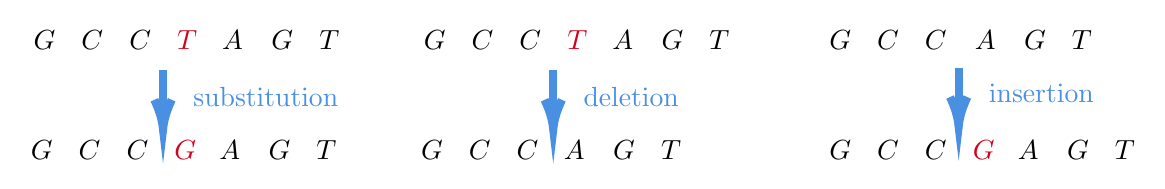
\begin{tikzpicture}[x=0.5pt,y=0.5pt,yscale=-1,xscale=1]
%uncomment if require: \path (0,146); %set diagram left start at 0, and has height of 146

%Straight Lines [id:da22824466810928623] 
\draw [color={rgb, 255:red, 74; green, 144; blue, 226 }  ,draw opacity=1 ][line width=3]    (110,43) -- (110,80) ;
\draw [shift={(110,85)}, rotate = 270] [color={rgb, 255:red, 74; green, 144; blue, 226 }  ,draw opacity=1 ][line width=3]    (20.77,-6.25) .. controls (13.2,-2.65) and (6.28,-0.57) .. (0,0) .. controls (6.28,0.57) and (13.2,2.66) .. (20.77,6.25)   ;
%Straight Lines [id:da021628931404131357] 
\draw [color={rgb, 255:red, 74; green, 144; blue, 226 }  ,draw opacity=1 ][line width=3]    (392,43) -- (392,80) ;
\draw [shift={(392,85)}, rotate = 270] [color={rgb, 255:red, 74; green, 144; blue, 226 }  ,draw opacity=1 ][line width=3]    (20.77,-6.25) .. controls (13.2,-2.65) and (6.28,-0.57) .. (0,0) .. controls (6.28,0.57) and (13.2,2.66) .. (20.77,6.25)   ;
%Straight Lines [id:da8581719584911228] 
\draw [color={rgb, 255:red, 74; green, 144; blue, 226 }  ,draw opacity=1 ][line width=3]    (685,41) -- (685,78) ;
\draw [shift={(685,83)}, rotate = 270] [color={rgb, 255:red, 74; green, 144; blue, 226 }  ,draw opacity=1 ][line width=3]    (20.77,-6.25) .. controls (13.2,-2.65) and (6.28,-0.57) .. (0,0) .. controls (6.28,0.57) and (13.2,2.66) .. (20.77,6.25)   ;

% Text Node
\draw (14.57,12.5) node [anchor=north west][inner sep=0.75pt]   [align=left] {$\displaystyle G$};
% Text Node
\draw (118.28,12.5) node [anchor=north west][inner sep=0.75pt]   [align=left] {$\displaystyle \textcolor[rgb]{0.82,0.01,0.11}{T}$};
% Text Node
\draw (49.14,12.5) node [anchor=north west][inner sep=0.75pt]   [align=left] {$\displaystyle C$};
% Text Node
\draw (150.85,12.5) node [anchor=north west][inner sep=0.75pt]   [align=left] {$\displaystyle A$};
% Text Node
\draw (186.42,12.5) node [anchor=north west][inner sep=0.75pt]   [align=left] {$\displaystyle G$};
% Text Node
\draw (83.71,12.5) node [anchor=north west][inner sep=0.75pt]   [align=left] {$\displaystyle C$};
% Text Node
\draw (221,12.5) node [anchor=north west][inner sep=0.75pt]   [align=left] {$\displaystyle T$};
% Text Node
\draw (12.57,91.5) node [anchor=north west][inner sep=0.75pt]   [align=left] {$\displaystyle G$};
% Text Node
\draw (116.28,91.5) node [anchor=north west][inner sep=0.75pt]   [align=left] {$\displaystyle \textcolor[rgb]{0.82,0.01,0.11}{G}$};
% Text Node
\draw (47.14,91.5) node [anchor=north west][inner sep=0.75pt]   [align=left] {$\displaystyle C$};
% Text Node
\draw (148.85,91.5) node [anchor=north west][inner sep=0.75pt]   [align=left] {$\displaystyle A$};
% Text Node
\draw (184.42,91.5) node [anchor=north west][inner sep=0.75pt]   [align=left] {$\displaystyle G$};
% Text Node
\draw (81.71,91.5) node [anchor=north west][inner sep=0.75pt]   [align=left] {$\displaystyle C$};
% Text Node
\draw (219,91.5) node [anchor=north west][inner sep=0.75pt]   [align=left] {$\displaystyle T$};
% Text Node
\draw (130,53) node [anchor=north west][inner sep=0.75pt]   [align=left] {\textcolor[rgb]{0.29,0.56,0.89}{substitution}};
% Text Node
\draw (296.57,12.5) node [anchor=north west][inner sep=0.75pt]   [align=left] {$\displaystyle G$};
% Text Node
\draw (400.28,12.5) node [anchor=north west][inner sep=0.75pt]   [align=left] {$\displaystyle \textcolor[rgb]{0.82,0.01,0.11}{T}$};
% Text Node
\draw (331.14,12.5) node [anchor=north west][inner sep=0.75pt]   [align=left] {$\displaystyle C$};
% Text Node
\draw (432.85,12.5) node [anchor=north west][inner sep=0.75pt]   [align=left] {$\displaystyle A$};
% Text Node
\draw (468.42,12.5) node [anchor=north west][inner sep=0.75pt]   [align=left] {$\displaystyle G$};
% Text Node
\draw (365.71,12.5) node [anchor=north west][inner sep=0.75pt]   [align=left] {$\displaystyle C$};
% Text Node
\draw (503,12.5) node [anchor=north west][inner sep=0.75pt]   [align=left] {$\displaystyle T$};
% Text Node
\draw (294.57,91.5) node [anchor=north west][inner sep=0.75pt]   [align=left] {$\displaystyle G$};
% Text Node
\draw (329.14,91.5) node [anchor=north west][inner sep=0.75pt]   [align=left] {$\displaystyle C$};
% Text Node
\draw (397.85,91.5) node [anchor=north west][inner sep=0.75pt]   [align=left] {$\displaystyle A$};
% Text Node
\draw (433.42,91.5) node [anchor=north west][inner sep=0.75pt]   [align=left] {$\displaystyle G$};
% Text Node
\draw (363.71,91.5) node [anchor=north west][inner sep=0.75pt]   [align=left] {$\displaystyle C$};
% Text Node
\draw (468,91.5) node [anchor=north west][inner sep=0.75pt]   [align=left] {$\displaystyle T$};
% Text Node
\draw (412,53) node [anchor=north west][inner sep=0.75pt]   [align=left] {\textcolor[rgb]{0.29,0.56,0.89}{deletion}};
% Text Node
\draw (589.57,12.5) node [anchor=north west][inner sep=0.75pt]   [align=left] {$\displaystyle G$};
% Text Node
\draw (624.14,12.5) node [anchor=north west][inner sep=0.75pt]   [align=left] {$\displaystyle C$};
% Text Node
\draw (694.85,12.5) node [anchor=north west][inner sep=0.75pt]   [align=left] {$\displaystyle A$};
% Text Node
\draw (730.42,12.5) node [anchor=north west][inner sep=0.75pt]   [align=left] {$\displaystyle G$};
% Text Node
\draw (658.71,12.5) node [anchor=north west][inner sep=0.75pt]   [align=left] {$\displaystyle C$};
% Text Node
\draw (765,12.5) node [anchor=north west][inner sep=0.75pt]   [align=left] {$\displaystyle T$};
% Text Node
\draw (705,51) node [anchor=north west][inner sep=0.75pt]   [align=left] {\textcolor[rgb]{0.29,0.56,0.89}{insertion}};
% Text Node
\draw (589.57,91.5) node [anchor=north west][inner sep=0.75pt]   [align=left] {$\displaystyle G$};
% Text Node
\draw (693.28,91.5) node [anchor=north west][inner sep=0.75pt]   [align=left] {$\displaystyle \textcolor[rgb]{0.82,0.01,0.11}{G}$};
% Text Node
\draw (624.14,91.5) node [anchor=north west][inner sep=0.75pt]   [align=left] {$\displaystyle C$};
% Text Node
\draw (725.85,91.5) node [anchor=north west][inner sep=0.75pt]   [align=left] {$\displaystyle A$};
% Text Node
\draw (761.42,91.5) node [anchor=north west][inner sep=0.75pt]   [align=left] {$\displaystyle G$};
% Text Node
\draw (658.71,91.5) node [anchor=north west][inner sep=0.75pt]   [align=left] {$\displaystyle C$};
% Text Node
\draw (796,91.5) node [anchor=north west][inner sep=0.75pt]   [align=left] {$\displaystyle T$};


\end{tikzpicture}

}
\caption{Illustration of the 3 types of mutation events in genome evolution.}
\label{fig:edits}
\end{figure}

An equivalent and convenient way to represent edits between two sequences 
is \emph{alignment}. See Figure~\ref{fig:align}.
In an alignment, deletions and insertions are represented with \emph{gaps}, shown with $-$.
(Note that deletions on $X$ is equivalent to insertions on $Y$;
deletions on $Y$ is equivalent to insertions on $X$.)
Both exactly-matched characters and mismatched-characters~(i.e., requires a substitutions event),
are shown by vertical-bars with substitutions highlighted.
Clearly, there is a one-to-one correspondence between a series
of events that transforms $X$ into $Y$ and an alignment between $X$ and $Y$,
and the number of events is equal to the number of gaps and mismatches in the alignment.
Hence, calculating edit distance between $X$ and $Y$ is equivalent to
seeking the optimal alignment between $X$ and $Y$~(here, ``optimal'' means
the number of gaps and mismatches in the alignment is minimized).

\begin{figure}[h]
\centering{

\tikzset{every picture/.style={line width=0.75pt}} %set default line width to 0.75pt        

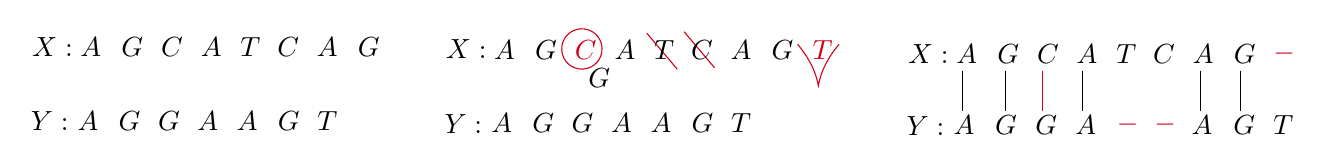
\begin{tikzpicture}[x=0.5pt,y=0.5pt,yscale=-1,xscale=1]
%uncomment if require: \path (0,146); %set diagram left start at 0, and has height of 146

%Straight Lines [id:da20102540282157666] 
\draw [color={rgb, 255:red, 208; green, 2; blue, 27 }  ,draw opacity=1 ]   (490,12) -- (512,38) ;
%Straight Lines [id:da009710943404266925] 
\draw [color={rgb, 255:red, 208; green, 2; blue, 27 }  ,draw opacity=1 ]   (463,13) -- (485,39) ;
%Shape: Circle [id:dp011981877187195566] 
\draw  [color={rgb, 255:red, 208; green, 2; blue, 27 }  ,draw opacity=1 ] (401.56,25.14) .. controls (401.15,17.1) and (407.35,10.25) .. (415.39,9.85) .. controls (423.43,9.45) and (430.28,15.64) .. (430.68,23.68) .. controls (431.09,31.73) and (424.89,38.57) .. (416.85,38.98) .. controls (408.81,39.38) and (401.96,33.19) .. (401.56,25.14) -- cycle ;
\draw  [color={rgb, 255:red, 208; green, 2; blue, 27 }  ,draw opacity=1 ] (602,21) .. controls (593.67,31) and (588.67,41) .. (587,51) .. controls (585.33,41) and (580.33,31) .. (572,21) ;
%Straight Lines [id:da5184853822717996] 
\draw    (691,40) -- (691,69) ;
%Straight Lines [id:da3211316725378842] 
\draw    (722,40) -- (722,69) ;
%Straight Lines [id:da18937901909445498] 
\draw [color={rgb, 255:red, 208; green, 2; blue, 27 }  ,draw opacity=1 ]   (749,40) -- (749,69) ;
%Straight Lines [id:da5526061509479675] 
\draw    (778,40) -- (778,69) ;
%Straight Lines [id:da6049458027827691] 
\draw    (863,40) -- (863,69) ;
%Straight Lines [id:da591487642150084] 
\draw    (892,40) -- (892,69) ;

% Text Node
\draw (81.5,14.5) node [anchor=north west][inner sep=0.75pt]   [align=left] {$\displaystyle G$};
% Text Node
\draw (167.45,14.5) node [anchor=north west][inner sep=0.75pt]   [align=left] {$\displaystyle \textcolor[rgb]{0,0,0}{T}$};
% Text Node
\draw (110.15,14.5) node [anchor=north west][inner sep=0.75pt]   [align=left] {$\displaystyle C$};
% Text Node
\draw (222.75,14.5) node [anchor=north west][inner sep=0.75pt]   [align=left] {$\displaystyle A$};
% Text Node
\draw (252.42,14.5) node [anchor=north west][inner sep=0.75pt]   [align=left] {$\displaystyle G$};
% Text Node
\draw (138.8,14.5) node [anchor=north west][inner sep=0.75pt]   [align=left] {$\displaystyle A$};
% Text Node
\draw (79.37,67.5) node [anchor=north west][inner sep=0.75pt]   [align=left] {$\displaystyle G$};
% Text Node
\draw (107.89,67.5) node [anchor=north west][inner sep=0.75pt]   [align=left] {$\displaystyle G$};
% Text Node
\draw (164.93,67.5) node [anchor=north west][inner sep=0.75pt]   [align=left] {$\displaystyle A$};
% Text Node
\draw (194.45,67.5) node [anchor=north west][inner sep=0.75pt]   [align=left] {$\displaystyle G$};
% Text Node
\draw (136.41,67.5) node [anchor=north west][inner sep=0.75pt]   [align=left] {$\displaystyle A$};
% Text Node
\draw (223,67.5) node [anchor=north west][inner sep=0.75pt]   [align=left] {$\displaystyle T$};
% Text Node
\draw (51.85,14.5) node [anchor=north west][inner sep=0.75pt]   [align=left] {$\displaystyle A$};
% Text Node
\draw (49.85,67.5) node [anchor=north west][inner sep=0.75pt]   [align=left] {$\displaystyle A$};
% Text Node
\draw (194.1,14.5) node [anchor=north west][inner sep=0.75pt]   [align=left] {$\displaystyle C$};
% Text Node
\draw (17,14) node [anchor=north west][inner sep=0.75pt]   [align=left] {$\displaystyle X:$};
% Text Node
\draw (16,68) node [anchor=north west][inner sep=0.75pt]   [align=left] {$\displaystyle Y:$};
% Text Node
\draw (380.5,16.5) node [anchor=north west][inner sep=0.75pt]   [align=left] {$\displaystyle G$};
% Text Node
\draw (466.45,16.5) node [anchor=north west][inner sep=0.75pt]   [align=left] {$\displaystyle \textcolor[rgb]{0,0,0}{T}$};
% Text Node
\draw (409.15,16.5) node [anchor=north west][inner sep=0.75pt]   [align=left] {$\displaystyle \textcolor[rgb]{0.82,0.01,0.11}{C}$};
% Text Node
\draw (521.75,16.5) node [anchor=north west][inner sep=0.75pt]   [align=left] {$\displaystyle A$};
% Text Node
\draw (551.42,16.5) node [anchor=north west][inner sep=0.75pt]   [align=left] {$\displaystyle G$};
% Text Node
\draw (437.8,16.5) node [anchor=north west][inner sep=0.75pt]   [align=left] {$\displaystyle A$};
% Text Node
\draw (378.37,69.5) node [anchor=north west][inner sep=0.75pt]   [align=left] {$\displaystyle G$};
% Text Node
\draw (406.89,69.5) node [anchor=north west][inner sep=0.75pt]   [align=left] {$\displaystyle G$};
% Text Node
\draw (463.93,69.5) node [anchor=north west][inner sep=0.75pt]   [align=left] {$\displaystyle A$};
% Text Node
\draw (493.45,69.5) node [anchor=north west][inner sep=0.75pt]   [align=left] {$\displaystyle G$};
% Text Node
\draw (435.41,69.5) node [anchor=north west][inner sep=0.75pt]   [align=left] {$\displaystyle A$};
% Text Node
\draw (522,69.5) node [anchor=north west][inner sep=0.75pt]   [align=left] {$\displaystyle T$};
% Text Node
\draw (350.85,16.5) node [anchor=north west][inner sep=0.75pt]   [align=left] {$\displaystyle A$};
% Text Node
\draw (348.85,69.5) node [anchor=north west][inner sep=0.75pt]   [align=left] {$\displaystyle A$};
% Text Node
\draw (493.1,16.5) node [anchor=north west][inner sep=0.75pt]   [align=left] {$\displaystyle C$};
% Text Node
\draw (316,16) node [anchor=north west][inner sep=0.75pt]   [align=left] {$\displaystyle X:$};
% Text Node
\draw (315,70) node [anchor=north west][inner sep=0.75pt]   [align=left] {$\displaystyle Y:$};
% Text Node
\draw (418.89,36.5) node [anchor=north west][inner sep=0.75pt]   [align=left] {$\displaystyle G$};
% Text Node
\draw (581,16.5) node [anchor=north west][inner sep=0.75pt]   [align=left] {$\displaystyle \textcolor[rgb]{0.82,0.01,0.11}{T}$};
% Text Node
\draw (714.5,19.25) node [anchor=north west][inner sep=0.75pt]   [align=left] {$\displaystyle G$};
% Text Node
\draw (800.45,19.25) node [anchor=north west][inner sep=0.75pt]   [align=left] {$\displaystyle \textcolor[rgb]{0,0,0}{T}$};
% Text Node
\draw (743.15,19.25) node [anchor=north west][inner sep=0.75pt]   [align=left] {$\displaystyle C$};
% Text Node
\draw (855.75,19.25) node [anchor=north west][inner sep=0.75pt]   [align=left] {$\displaystyle A$};
% Text Node
\draw (885.42,19.25) node [anchor=north west][inner sep=0.75pt]   [align=left] {$\displaystyle G$};
% Text Node
\draw (771.8,19.25) node [anchor=north west][inner sep=0.75pt]   [align=left] {$\displaystyle A$};
% Text Node
\draw (712.87,70.75) node [anchor=north west][inner sep=0.75pt]   [align=left] {$\displaystyle G$};
% Text Node
\draw (741.89,70.75) node [anchor=north west][inner sep=0.75pt]   [align=left] {$\displaystyle G$};
% Text Node
\draw (854.97,70.75) node [anchor=north west][inner sep=0.75pt]   [align=left] {$\displaystyle A$};
% Text Node
\draw (884.99,70.75) node [anchor=north west][inner sep=0.75pt]   [align=left] {$\displaystyle G$};
% Text Node
\draw (770.91,70.75) node [anchor=north west][inner sep=0.75pt]   [align=left] {$\displaystyle A$};
% Text Node
\draw (914,70.75) node [anchor=north west][inner sep=0.75pt]   [align=left] {$\displaystyle T$};
% Text Node
\draw (684.85,19.25) node [anchor=north west][inner sep=0.75pt]   [align=left] {$\displaystyle A$};
% Text Node
\draw (682.85,70.75) node [anchor=north west][inner sep=0.75pt]   [align=left] {$\displaystyle A$};
% Text Node
\draw (827.1,19.25) node [anchor=north west][inner sep=0.75pt]   [align=left] {$\displaystyle C$};
% Text Node
\draw (650,19.25) node [anchor=north west][inner sep=0.75pt]   [align=left] {$\displaystyle X:$};
% Text Node
\draw (649,71.25) node [anchor=north west][inner sep=0.75pt]   [align=left] {$\displaystyle Y:$};
% Text Node
\draw (800.93,70.75) node [anchor=north west][inner sep=0.75pt]   [align=left] {$\displaystyle \textcolor[rgb]{0.82,0.01,0.11}{-}$};
% Text Node
\draw (827.95,70.75) node [anchor=north west][inner sep=0.75pt]   [align=left] {$\displaystyle \textcolor[rgb]{0.82,0.01,0.11}{-}$};
% Text Node
\draw (913.89,19.25) node [anchor=north west][inner sep=0.75pt]   [align=left] {$\displaystyle \textcolor[rgb]{0.82,0.01,0.11}{-}$};


\end{tikzpicture}

}
\caption{Illustration of the edit distance and the corresponding optimal alignment.}
\label{fig:align}
\end{figure}


\subsection*{The Algorithm}

We now design a dynamic programming to find the optimal alignment of two given strings.
We first look into the optimal substructures. Suppose that $\mathcal{A}$ is the optimal
alignment of two strings $X$ and $Y$~(see Figure~\ref{fig:optimal}).
Then clearly its substructure, i.e., the first $k$ columns, gives the optimal
alignment between the corresponding two substrings, which can be obtained by removing
the gaps in the first $k$ columns of $\mathcal{A}$.
(Proof: if the two substrings can be aligned with
a better alignment~(with smaller number of gaps and mismatches), then we can have
a better alignment, than $\mathcal{A}$, between $X$ and $Y$,
by concatenating to it the remaining columns of $\mathcal{A}$.)

\begin{figure}[h]
\centering{

\tikzset{every picture/.style={line width=0.75pt}} %set default line width to 0.75pt        

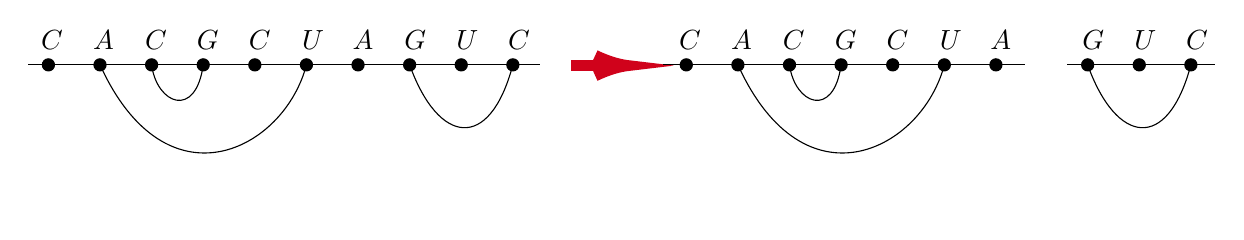
\begin{tikzpicture}[x=0.5pt,y=0.5pt,yscale=-1,xscale=1]
%uncomment if require: \path (0,118); %set diagram left start at 0, and has height of 118

%Flowchart: Connector [id:dp8000065927198341] 
\draw  [fill={rgb, 255:red, 0; green, 0; blue, 0 }  ,fill opacity=1 ] (25,40.9) .. controls (25.87,38.65) and (28.4,37.52) .. (30.66,38.39) .. controls (32.91,39.26) and (34.04,41.79) .. (33.17,44.05) .. controls (32.3,46.3) and (29.77,47.43) .. (27.51,46.56) .. controls (25.26,45.69) and (24.13,43.16) .. (25,40.9) -- cycle ;
%Flowchart: Connector [id:dp15246894411278777] 
\draw  [fill={rgb, 255:red, 0; green, 0; blue, 0 }  ,fill opacity=1 ] (62.3,40.9) .. controls (63.16,38.65) and (65.7,37.52) .. (67.95,38.39) .. controls (70.21,39.26) and (71.33,41.79) .. (70.46,44.05) .. controls (69.59,46.3) and (67.06,47.43) .. (64.81,46.56) .. controls (62.55,45.69) and (61.43,43.16) .. (62.3,40.9) -- cycle ;
%Flowchart: Connector [id:dp36869196941163607] 
\draw  [fill={rgb, 255:red, 0; green, 0; blue, 0 }  ,fill opacity=1 ] (99.59,40.9) .. controls (100.46,38.65) and (102.99,37.52) .. (105.25,38.39) .. controls (107.5,39.26) and (108.63,41.79) .. (107.76,44.05) .. controls (106.89,46.3) and (104.36,47.43) .. (102.1,46.56) .. controls (99.85,45.69) and (98.72,43.16) .. (99.59,40.9) -- cycle ;
%Flowchart: Connector [id:dp16694338209837356] 
\draw  [fill={rgb, 255:red, 0; green, 0; blue, 0 }  ,fill opacity=1 ] (136.89,40.9) .. controls (137.75,38.65) and (140.29,37.52) .. (142.54,38.39) .. controls (144.8,39.26) and (145.92,41.79) .. (145.05,44.05) .. controls (144.18,46.3) and (141.65,47.43) .. (139.4,46.56) .. controls (137.14,45.69) and (136.02,43.16) .. (136.89,40.9) -- cycle ;
%Flowchart: Connector [id:dp42963486447916044] 
\draw  [fill={rgb, 255:red, 0; green, 0; blue, 0 }  ,fill opacity=1 ] (174.18,40.9) .. controls (175.05,38.65) and (177.58,37.52) .. (179.84,38.39) .. controls (182.09,39.26) and (183.22,41.79) .. (182.35,44.05) .. controls (181.48,46.3) and (178.95,47.43) .. (176.69,46.56) .. controls (174.44,45.69) and (173.31,43.16) .. (174.18,40.9) -- cycle ;
%Flowchart: Connector [id:dp5506217339056906] 
\draw  [fill={rgb, 255:red, 0; green, 0; blue, 0 }  ,fill opacity=1 ] (211.48,40.9) .. controls (212.34,38.65) and (214.88,37.52) .. (217.13,38.39) .. controls (219.39,39.26) and (220.51,41.79) .. (219.64,44.05) .. controls (218.77,46.3) and (216.24,47.43) .. (213.99,46.56) .. controls (211.73,45.69) and (210.61,43.16) .. (211.48,40.9) -- cycle ;
%Flowchart: Connector [id:dp9698798449909987] 
\draw  [fill={rgb, 255:red, 0; green, 0; blue, 0 }  ,fill opacity=1 ] (248.77,40.9) .. controls (249.64,38.65) and (252.17,37.52) .. (254.43,38.39) .. controls (256.68,39.26) and (257.81,41.79) .. (256.94,44.05) .. controls (256.07,46.3) and (253.54,47.43) .. (251.28,46.56) .. controls (249.03,45.69) and (247.9,43.16) .. (248.77,40.9) -- cycle ;
%Flowchart: Connector [id:dp6216415603842047] 
\draw  [fill={rgb, 255:red, 0; green, 0; blue, 0 }  ,fill opacity=1 ] (286.07,40.9) .. controls (286.93,38.65) and (289.47,37.52) .. (291.72,38.39) .. controls (293.98,39.26) and (295.1,41.79) .. (294.23,44.05) .. controls (293.36,46.3) and (290.83,47.43) .. (288.58,46.56) .. controls (286.32,45.69) and (285.2,43.16) .. (286.07,40.9) -- cycle ;
%Flowchart: Connector [id:dp3011581402055178] 
\draw  [fill={rgb, 255:red, 0; green, 0; blue, 0 }  ,fill opacity=1 ] (323.36,40.9) .. controls (324.23,38.65) and (326.76,37.52) .. (329.02,38.39) .. controls (331.27,39.26) and (332.4,41.79) .. (331.53,44.05) .. controls (330.66,46.3) and (328.13,47.43) .. (325.87,46.56) .. controls (323.62,45.69) and (322.49,43.16) .. (323.36,40.9) -- cycle ;
%Flowchart: Connector [id:dp9886740109361196] 
\draw  [fill={rgb, 255:red, 0; green, 0; blue, 0 }  ,fill opacity=1 ] (360.66,40.9) .. controls (361.52,38.65) and (364.06,37.52) .. (366.31,38.39) .. controls (368.57,39.26) and (369.69,41.79) .. (368.82,44.05) .. controls (367.95,46.3) and (365.42,47.43) .. (363.17,46.56) .. controls (360.91,45.69) and (359.79,43.16) .. (360.66,40.9) -- cycle ;
%Straight Lines [id:da7380690811587965] 
\draw    (14.5,42.48) -- (384.5,42.48) ;
%Curve Lines [id:da5249448376389138] 
\draw    (66.38,42.48) .. controls (114.5,148) and (199.5,104) .. (215.56,42.48) ;
%Curve Lines [id:da6743430437445295] 
\draw    (103.67,42.48) .. controls (107.5,71) and (135.5,82) .. (140.97,42.48) ;
%Curve Lines [id:da22021299625417579] 
\draw    (290.15,42.48) .. controls (310.8,100) and (347.8,106) .. (364.74,42.48) ;
%Straight Lines [id:da7069209190780016] 
\draw [color={rgb, 255:red, 208; green, 2; blue, 27 }  ,draw opacity=1 ][line width=3.75]    (407,43) -- (443.5,43) ;
\draw [shift={(449.5,43)}, rotate = 180] [color={rgb, 255:red, 208; green, 2; blue, 27 }  ,draw opacity=1 ][line width=3.75]    (25.14,-7.57) .. controls (15.99,-3.21) and (7.61,-0.69) .. (0,0) .. controls (7.61,0.69) and (15.99,3.21) .. (25.14,7.57)   ;
%Flowchart: Connector [id:dp5322197909537895] 
\draw  [fill={rgb, 255:red, 0; green, 0; blue, 0 }  ,fill opacity=1 ] (776.07,40.9) .. controls (776.93,38.65) and (779.47,37.52) .. (781.72,38.39) .. controls (783.98,39.26) and (785.1,41.79) .. (784.23,44.05) .. controls (783.36,46.3) and (780.83,47.43) .. (778.58,46.56) .. controls (776.32,45.69) and (775.2,43.16) .. (776.07,40.9) -- cycle ;
%Flowchart: Connector [id:dp13352675314788975] 
\draw  [fill={rgb, 255:red, 0; green, 0; blue, 0 }  ,fill opacity=1 ] (813.36,40.9) .. controls (814.23,38.65) and (816.76,37.52) .. (819.02,38.39) .. controls (821.27,39.26) and (822.4,41.79) .. (821.53,44.05) .. controls (820.66,46.3) and (818.13,47.43) .. (815.87,46.56) .. controls (813.62,45.69) and (812.49,43.16) .. (813.36,40.9) -- cycle ;
%Flowchart: Connector [id:dp21192888942378674] 
\draw  [fill={rgb, 255:red, 0; green, 0; blue, 0 }  ,fill opacity=1 ] (850.66,40.9) .. controls (851.52,38.65) and (854.06,37.52) .. (856.31,38.39) .. controls (858.57,39.26) and (859.69,41.79) .. (858.82,44.05) .. controls (857.95,46.3) and (855.42,47.43) .. (853.17,46.56) .. controls (850.91,45.69) and (849.79,43.16) .. (850.66,40.9) -- cycle ;
%Straight Lines [id:da824569447163987] 
\draw    (765.5,42.48) -- (872.5,42.48) ;
%Curve Lines [id:da7044902821535391] 
\draw    (780.15,42.48) .. controls (800.8,100) and (837.8,106) .. (854.74,42.48) ;
%Flowchart: Connector [id:dp9350094771084225] 
\draw  [fill={rgb, 255:red, 0; green, 0; blue, 0 }  ,fill opacity=1 ] (486,40.9) .. controls (486.87,38.65) and (489.4,37.52) .. (491.66,38.39) .. controls (493.91,39.26) and (495.04,41.79) .. (494.17,44.05) .. controls (493.3,46.3) and (490.77,47.43) .. (488.51,46.56) .. controls (486.26,45.69) and (485.13,43.16) .. (486,40.9) -- cycle ;
%Flowchart: Connector [id:dp11350907508532626] 
\draw  [fill={rgb, 255:red, 0; green, 0; blue, 0 }  ,fill opacity=1 ] (523.3,40.9) .. controls (524.16,38.65) and (526.7,37.52) .. (528.95,38.39) .. controls (531.21,39.26) and (532.33,41.79) .. (531.46,44.05) .. controls (530.59,46.3) and (528.06,47.43) .. (525.81,46.56) .. controls (523.55,45.69) and (522.43,43.16) .. (523.3,40.9) -- cycle ;
%Flowchart: Connector [id:dp3052785983719639] 
\draw  [fill={rgb, 255:red, 0; green, 0; blue, 0 }  ,fill opacity=1 ] (560.59,40.9) .. controls (561.46,38.65) and (563.99,37.52) .. (566.25,38.39) .. controls (568.5,39.26) and (569.63,41.79) .. (568.76,44.05) .. controls (567.89,46.3) and (565.36,47.43) .. (563.1,46.56) .. controls (560.85,45.69) and (559.72,43.16) .. (560.59,40.9) -- cycle ;
%Flowchart: Connector [id:dp03710718088561116] 
\draw  [fill={rgb, 255:red, 0; green, 0; blue, 0 }  ,fill opacity=1 ] (597.89,40.9) .. controls (598.75,38.65) and (601.29,37.52) .. (603.54,38.39) .. controls (605.8,39.26) and (606.92,41.79) .. (606.05,44.05) .. controls (605.18,46.3) and (602.65,47.43) .. (600.4,46.56) .. controls (598.14,45.69) and (597.02,43.16) .. (597.89,40.9) -- cycle ;
%Flowchart: Connector [id:dp23670841860659286] 
\draw  [fill={rgb, 255:red, 0; green, 0; blue, 0 }  ,fill opacity=1 ] (635.18,40.9) .. controls (636.05,38.65) and (638.58,37.52) .. (640.84,38.39) .. controls (643.09,39.26) and (644.22,41.79) .. (643.35,44.05) .. controls (642.48,46.3) and (639.95,47.43) .. (637.69,46.56) .. controls (635.44,45.69) and (634.31,43.16) .. (635.18,40.9) -- cycle ;
%Flowchart: Connector [id:dp22400416886884278] 
\draw  [fill={rgb, 255:red, 0; green, 0; blue, 0 }  ,fill opacity=1 ] (672.48,40.9) .. controls (673.34,38.65) and (675.88,37.52) .. (678.13,38.39) .. controls (680.39,39.26) and (681.51,41.79) .. (680.64,44.05) .. controls (679.77,46.3) and (677.24,47.43) .. (674.99,46.56) .. controls (672.73,45.69) and (671.61,43.16) .. (672.48,40.9) -- cycle ;
%Flowchart: Connector [id:dp3681462959706371] 
\draw  [fill={rgb, 255:red, 0; green, 0; blue, 0 }  ,fill opacity=1 ] (709.77,40.9) .. controls (710.64,38.65) and (713.17,37.52) .. (715.43,38.39) .. controls (717.68,39.26) and (718.81,41.79) .. (717.94,44.05) .. controls (717.07,46.3) and (714.54,47.43) .. (712.28,46.56) .. controls (710.03,45.69) and (708.9,43.16) .. (709.77,40.9) -- cycle ;
%Straight Lines [id:da2794395954613992] 
\draw    (473.5,42.48) -- (734.5,42.48) ;
%Curve Lines [id:da2506737550157674] 
\draw    (527.38,42.48) .. controls (575.5,148) and (660.5,104) .. (676.56,42.48) ;
%Curve Lines [id:da25133040404462803] 
\draw    (564.67,42.48) .. controls (568.5,71) and (596.5,82) .. (601.97,42.48) ;

% Text Node
\draw (22,16) node [anchor=north west][inner sep=0.75pt]   [align=left] {$\displaystyle C$};
% Text Node
\draw (59.5,16) node [anchor=north west][inner sep=0.75pt]   [align=left] {$\displaystyle A$};
% Text Node
\draw (97,16) node [anchor=north west][inner sep=0.75pt]   [align=left] {$\displaystyle C$};
% Text Node
\draw (134.5,16) node [anchor=north west][inner sep=0.75pt]   [align=left] {$\displaystyle G$};
% Text Node
\draw (172,16) node [anchor=north west][inner sep=0.75pt]   [align=left] {$\displaystyle C$};
% Text Node
\draw (210.5,16) node [anchor=north west][inner sep=0.75pt]   [align=left] {$\displaystyle U$};
% Text Node
\draw (247,16) node [anchor=north west][inner sep=0.75pt]   [align=left] {$\displaystyle A$};
% Text Node
\draw (322,16) node [anchor=north west][inner sep=0.75pt]   [align=left] {$\displaystyle U$};
% Text Node
\draw (359.48,16) node [anchor=north west][inner sep=0.75pt]   [align=left] {$\displaystyle C$};
% Text Node
\draw (284.5,16) node [anchor=north west][inner sep=0.75pt]   [align=left] {$\displaystyle G$};
% Text Node
\draw (812,16) node [anchor=north west][inner sep=0.75pt]   [align=left] {$\displaystyle U$};
% Text Node
\draw (849.48,16) node [anchor=north west][inner sep=0.75pt]   [align=left] {$\displaystyle C$};
% Text Node
\draw (774.5,16) node [anchor=north west][inner sep=0.75pt]   [align=left] {$\displaystyle G$};
% Text Node
\draw (483,16) node [anchor=north west][inner sep=0.75pt]   [align=left] {$\displaystyle C$};
% Text Node
\draw (520.5,16) node [anchor=north west][inner sep=0.75pt]   [align=left] {$\displaystyle A$};
% Text Node
\draw (558,16) node [anchor=north west][inner sep=0.75pt]   [align=left] {$\displaystyle C$};
% Text Node
\draw (595.5,16) node [anchor=north west][inner sep=0.75pt]   [align=left] {$\displaystyle G$};
% Text Node
\draw (633,16) node [anchor=north west][inner sep=0.75pt]   [align=left] {$\displaystyle C$};
% Text Node
\draw (671.5,16) node [anchor=north west][inner sep=0.75pt]   [align=left] {$\displaystyle U$};
% Text Node
\draw (708,16) node [anchor=north west][inner sep=0.75pt]   [align=left] {$\displaystyle A$};


\end{tikzpicture}

}
\caption{Illustration of the optimal substructure of alignment.
The left figure shows the optimal alignment between $X$ and $Y$.
Then we can remove any number of columns from right-side, and the resulting
alignment must be the optimal alignment of the corresponding two substrings.
For examples, the middle figure shows the optimal alignment between $X' = AGCATCAG$ and $Y' = AGGAAG$,
where one column of the alignment in the left-figure is removed;
and the right figure shows the optimal alignment between $X'' = AGCATC$ and $Y'' = AGGA$,
where three columns of the alignment in the left-figure is removed.}
\label{fig:optimal}
\end{figure}

So, the alignment problem indeed satisfies the optimal substructure property.
And the substructure suggests defining the subproblems as to computing the optimal
alignment between a substring of $X$~(starting from beginning) and 
a substring of $Y$~(starting from beginning).
Formally, let $F(i,j)$ be the edit distance between $X[1\cdots i]$ and $Y[1\cdots j]$.
Clearly, we have $d(X, Y) = F(|X|, |Y|)$.
Now we develop a recursion. In order to calculate the optimal alignment between $X[1\cdots i]$
and $Y[1\cdots j]$, consider the possible scenario of the last step, i.e., how $X[i]$ and $X[j]$
are placed in the optimal alignment. There are three cases. See Figure~\ref{fig:recursion}.

\begin{figure}[h]
\centering{

\tikzset{every picture/.style={line width=0.75pt}} %set default line width to 0.75pt        

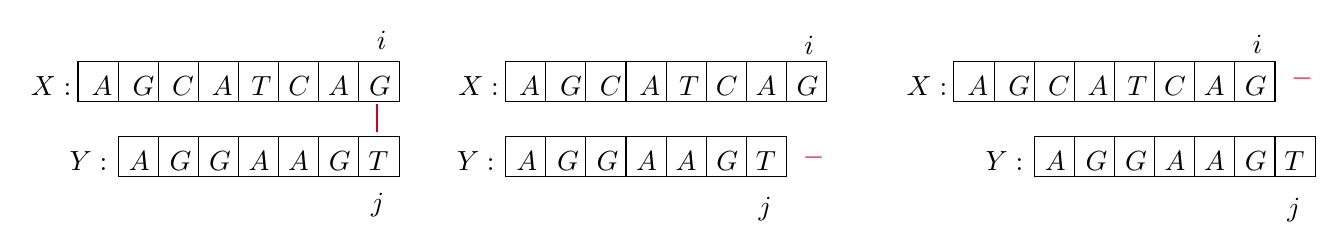
\begin{tikzpicture}[x=0.5pt,y=0.5pt,yscale=-1,xscale=1]
%uncomment if require: \path (0,172); %set diagram left start at 0, and has height of 172

%Straight Lines [id:da5184853822717996] 
\draw [color={rgb, 255:red, 208; green, 2; blue, 27 }  ,draw opacity=1 ][line width=0.75]    (265,71) -- (265,91) ;
%Shape: Grid [id:dp39994906595632274] 
\draw  [draw opacity=0] (49,40) -- (281,40) -- (281,69) -- (49,69) -- cycle ; \draw   (78,40) -- (78,69)(107,40) -- (107,69)(136,40) -- (136,69)(165,40) -- (165,69)(194,40) -- (194,69)(223,40) -- (223,69)(252,40) -- (252,69) ; \draw    ; \draw   (49,40) -- (281,40) -- (281,69) -- (49,69) -- cycle ;
%Shape: Grid [id:dp8100536729244665] 
\draw  [draw opacity=0] (78,94) -- (281,94) -- (281,123) -- (78,123) -- cycle ; \draw   (107,94) -- (107,123)(136,94) -- (136,123)(165,94) -- (165,123)(194,94) -- (194,123)(223,94) -- (223,123)(252,94) -- (252,123) ; \draw    ; \draw   (78,94) -- (281,94) -- (281,123) -- (78,123) -- cycle ;
%Shape: Grid [id:dp4933742529886569] 
\draw  [draw opacity=0] (358,40) -- (590,40) -- (590,69) -- (358,69) -- cycle ; \draw   (387,40) -- (387,69)(416,40) -- (416,69)(445,40) -- (445,69)(474,40) -- (474,69)(503,40) -- (503,69)(532,40) -- (532,69)(561,40) -- (561,69) ; \draw    ; \draw   (358,40) -- (590,40) -- (590,69) -- (358,69) -- cycle ;
%Shape: Grid [id:dp3002745379875943] 
\draw  [draw opacity=0] (358,94) -- (561,94) -- (561,123) -- (358,123) -- cycle ; \draw   (387,94) -- (387,123)(416,94) -- (416,123)(445,94) -- (445,123)(474,94) -- (474,123)(503,94) -- (503,123)(532,94) -- (532,123) ; \draw    ; \draw   (358,94) -- (561,94) -- (561,123) -- (358,123) -- cycle ;
%Shape: Grid [id:dp20349177163511312] 
\draw  [draw opacity=0] (682,40) -- (914,40) -- (914,69) -- (682,69) -- cycle ; \draw   (711,40) -- (711,69)(740,40) -- (740,69)(769,40) -- (769,69)(798,40) -- (798,69)(827,40) -- (827,69)(856,40) -- (856,69)(885,40) -- (885,69) ; \draw    ; \draw   (682,40) -- (914,40) -- (914,69) -- (682,69) -- cycle ;
%Shape: Grid [id:dp02508286059103748] 
\draw  [draw opacity=0] (740,94) -- (943,94) -- (943,123) -- (740,123) -- cycle ; \draw   (769,94) -- (769,123)(798,94) -- (798,123)(827,94) -- (827,123)(856,94) -- (856,123)(885,94) -- (885,123)(914,94) -- (914,123) ; \draw    ; \draw   (740,94) -- (943,94) -- (943,123) -- (740,123) -- cycle ;

% Text Node
\draw (86.5,49) node [anchor=north west][inner sep=0.75pt]   [align=left] {$\displaystyle G$};
% Text Node
\draw (172.45,49) node [anchor=north west][inner sep=0.75pt]   [align=left] {$\displaystyle \textcolor[rgb]{0,0,0}{T}$};
% Text Node
\draw (115.15,49) node [anchor=north west][inner sep=0.75pt]   [align=left] {$\displaystyle C$};
% Text Node
\draw (227.75,49) node [anchor=north west][inner sep=0.75pt]   [align=left] {$\displaystyle A$};
% Text Node
\draw (257.42,49) node [anchor=north west][inner sep=0.75pt]   [align=left] {$\displaystyle G$};
% Text Node
\draw (143.8,49) node [anchor=north west][inner sep=0.75pt]   [align=left] {$\displaystyle A$};
% Text Node
\draw (113.37,103) node [anchor=north west][inner sep=0.75pt]   [align=left] {$\displaystyle G$};
% Text Node
\draw (141.89,103) node [anchor=north west][inner sep=0.75pt]   [align=left] {$\displaystyle G$};
% Text Node
\draw (198.93,103) node [anchor=north west][inner sep=0.75pt]   [align=left] {$\displaystyle A$};
% Text Node
\draw (228.45,103) node [anchor=north west][inner sep=0.75pt]   [align=left] {$\displaystyle G$};
% Text Node
\draw (170.41,103) node [anchor=north west][inner sep=0.75pt]   [align=left] {$\displaystyle A$};
% Text Node
\draw (257,103) node [anchor=north west][inner sep=0.75pt]   [align=left] {$\displaystyle T$};
% Text Node
\draw (56.85,49) node [anchor=north west][inner sep=0.75pt]   [align=left] {$\displaystyle A$};
% Text Node
\draw (83.85,103) node [anchor=north west][inner sep=0.75pt]   [align=left] {$\displaystyle A$};
% Text Node
\draw (199.1,49) node [anchor=north west][inner sep=0.75pt]   [align=left] {$\displaystyle C$};
% Text Node
\draw (13,49) node [anchor=north west][inner sep=0.75pt]   [align=left] {$\displaystyle X:$};
% Text Node
\draw (41,103) node [anchor=north west][inner sep=0.75pt]   [align=left] {$\displaystyle Y:$};
% Text Node
\draw (263,16) node [anchor=north west][inner sep=0.75pt]   [align=left] {$\displaystyle i$};
% Text Node
\draw (259,133) node [anchor=north west][inner sep=0.75pt]   [align=left] {$\displaystyle j$};
% Text Node
\draw (395.5,49) node [anchor=north west][inner sep=0.75pt]   [align=left] {$\displaystyle G$};
% Text Node
\draw (481.45,49) node [anchor=north west][inner sep=0.75pt]   [align=left] {$\displaystyle \textcolor[rgb]{0,0,0}{T}$};
% Text Node
\draw (424.15,49) node [anchor=north west][inner sep=0.75pt]   [align=left] {$\displaystyle C$};
% Text Node
\draw (536.75,49) node [anchor=north west][inner sep=0.75pt]   [align=left] {$\displaystyle A$};
% Text Node
\draw (566.42,49) node [anchor=north west][inner sep=0.75pt]   [align=left] {$\displaystyle G$};
% Text Node
\draw (452.8,49) node [anchor=north west][inner sep=0.75pt]   [align=left] {$\displaystyle A$};
% Text Node
\draw (393.37,103) node [anchor=north west][inner sep=0.75pt]   [align=left] {$\displaystyle G$};
% Text Node
\draw (421.89,103) node [anchor=north west][inner sep=0.75pt]   [align=left] {$\displaystyle G$};
% Text Node
\draw (478.93,103) node [anchor=north west][inner sep=0.75pt]   [align=left] {$\displaystyle A$};
% Text Node
\draw (508.45,103) node [anchor=north west][inner sep=0.75pt]   [align=left] {$\displaystyle G$};
% Text Node
\draw (450.41,103) node [anchor=north west][inner sep=0.75pt]   [align=left] {$\displaystyle A$};
% Text Node
\draw (537,103) node [anchor=north west][inner sep=0.75pt]   [align=left] {$\displaystyle T$};
% Text Node
\draw (365.85,49) node [anchor=north west][inner sep=0.75pt]   [align=left] {$\displaystyle A$};
% Text Node
\draw (363.85,103) node [anchor=north west][inner sep=0.75pt]   [align=left] {$\displaystyle A$};
% Text Node
\draw (508.1,49) node [anchor=north west][inner sep=0.75pt]   [align=left] {$\displaystyle C$};
% Text Node
\draw (322,49) node [anchor=north west][inner sep=0.75pt]   [align=left] {$\displaystyle X:$};
% Text Node
\draw (321,103) node [anchor=north west][inner sep=0.75pt]   [align=left] {$\displaystyle Y:$};
% Text Node
\draw (572,20) node [anchor=north west][inner sep=0.75pt]   [align=left] {$\displaystyle i$};
% Text Node
\draw (539,136) node [anchor=north west][inner sep=0.75pt]   [align=left] {$\displaystyle j$};
% Text Node
\draw (570.93,101) node [anchor=north west][inner sep=0.75pt]   [align=left] {$\displaystyle \textcolor[rgb]{0.82,0.01,0.11}{-}$};
% Text Node
\draw (719.5,49) node [anchor=north west][inner sep=0.75pt]   [align=left] {$\displaystyle G$};
% Text Node
\draw (805.45,49) node [anchor=north west][inner sep=0.75pt]   [align=left] {$\displaystyle \textcolor[rgb]{0,0,0}{T}$};
% Text Node
\draw (748.15,49) node [anchor=north west][inner sep=0.75pt]   [align=left] {$\displaystyle C$};
% Text Node
\draw (860.75,49) node [anchor=north west][inner sep=0.75pt]   [align=left] {$\displaystyle A$};
% Text Node
\draw (890.42,49) node [anchor=north west][inner sep=0.75pt]   [align=left] {$\displaystyle G$};
% Text Node
\draw (776.8,49) node [anchor=north west][inner sep=0.75pt]   [align=left] {$\displaystyle A$};
% Text Node
\draw (775.37,103) node [anchor=north west][inner sep=0.75pt]   [align=left] {$\displaystyle G$};
% Text Node
\draw (803.89,103) node [anchor=north west][inner sep=0.75pt]   [align=left] {$\displaystyle G$};
% Text Node
\draw (860.93,103) node [anchor=north west][inner sep=0.75pt]   [align=left] {$\displaystyle A$};
% Text Node
\draw (890.45,103) node [anchor=north west][inner sep=0.75pt]   [align=left] {$\displaystyle G$};
% Text Node
\draw (832.41,103) node [anchor=north west][inner sep=0.75pt]   [align=left] {$\displaystyle A$};
% Text Node
\draw (919,103) node [anchor=north west][inner sep=0.75pt]   [align=left] {$\displaystyle T$};
% Text Node
\draw (689.85,49) node [anchor=north west][inner sep=0.75pt]   [align=left] {$\displaystyle A$};
% Text Node
\draw (745.85,103) node [anchor=north west][inner sep=0.75pt]   [align=left] {$\displaystyle A$};
% Text Node
\draw (832.1,49) node [anchor=north west][inner sep=0.75pt]   [align=left] {$\displaystyle C$};
% Text Node
\draw (646,49) node [anchor=north west][inner sep=0.75pt]   [align=left] {$\displaystyle X:$};
% Text Node
\draw (703,103) node [anchor=north west][inner sep=0.75pt]   [align=left] {$\displaystyle Y:$};
% Text Node
\draw (896,19) node [anchor=north west][inner sep=0.75pt]   [align=left] {$\displaystyle i$};
% Text Node
\draw (921,137) node [anchor=north west][inner sep=0.75pt]   [align=left] {$\displaystyle j$};
% Text Node
\draw (923.93,44) node [anchor=north west][inner sep=0.75pt]   [align=left] {$\displaystyle \textcolor[rgb]{0.82,0.01,0.11}{-}$};


\end{tikzpicture}

}
\caption{Illustration of the three cases in developing the recursion.}
\label{fig:recursion}
\end{figure}


First, $X[i]$ is aligned to $Y[j]$ in the optimal alignment. In this case, the optimal alignment
between $X[1\cdots i]$ and $Y[1\cdots j]$ can be obtained by concatenating the optimal alignment
between $X[1\cdots i-1]$ and $Y[1\cdots j-1]$ and this column of $(X[i], Y[j])^T$.
Hence, in this case, $F(i,j) = F(i, j) + \delta(X[i] \neq Y[j])$, where the delta function
$\delta(X[i] \neq Y[j]) = 1$ if $X[i] \neq Y[j]$, i.e., a mismatch that requires a substitution event,
and $\delta(X[i] \neq Y[j]) = 0$ if $X[i] = Y[j]$, i.e., an exactly-match that does not need any event.
%The extra delta function represents if a substitution is needed.

Second, $X[i]$ is not aligned~(or, aligned to a gap) in the optimal alignment. In this case, the optimal alignment
between $X[1\cdots i]$ and $Y[1\cdots j]$ can be obtained by concatenating the optimal alignment
between $X[1\cdots i-1]$ and $Y[1\cdots j]$ and this column of $(X[i], -)^T$.
Hence, in this case, $F(i,j) = F(i-1, j) + 1$, where 
the extra 1 represents a deletion on $X$ is needed.

Third, $Y[j]$ is not aligned~(or, aligned to a gap) in the optimal alignment. In this case, the optimal alignment
between $X[1\cdots i]$ and $Y[1\cdots j]$ can be obtained by concatenating the optimal alignment
between $X[1\cdots i]$ and $Y[1\cdots j-1]$ and this column of $(-, Y[j])^T$.
Hence, in this case, $F(i,j) = F(i, j- 1) + 1$, where 
the extra 1 represents a deletion on $Y$ is needed.

Combined, the recursion is given below.
\begin{displaymath}
F(i,j) = \min\left\{
	\begin{array}{llll}
	F(i-1,j-1) + \delta(X[i] \neq Y[j]) \\
	F(i-1,j) + 1 \\
	F(i,j-1) + 1 \\
	\end{array}
\right.
\end{displaymath}

We now can complete the algorithm. The algorithm fills a DP table. See Figure~\ref{fig:table}.
To facilitate the recursion, we add a new row and a new column in the table,
and fill them in the initialization step. 
We then fill the table, either row by row, or column by column~(why both work?).
The right bottom entry, $F(|X|, |Y|)$, gives the edit distance between $X$ and $Y$.
The actual alignment can be constructed by maintaining a tracking back pointer on each entry.
The running time of the algorithm is therefore $O(|X||Y|)$.

\begin{figure}[h]
\centering{

\tikzset{every picture/.style={line width=0.75pt}} %set default line width to 0.75pt        

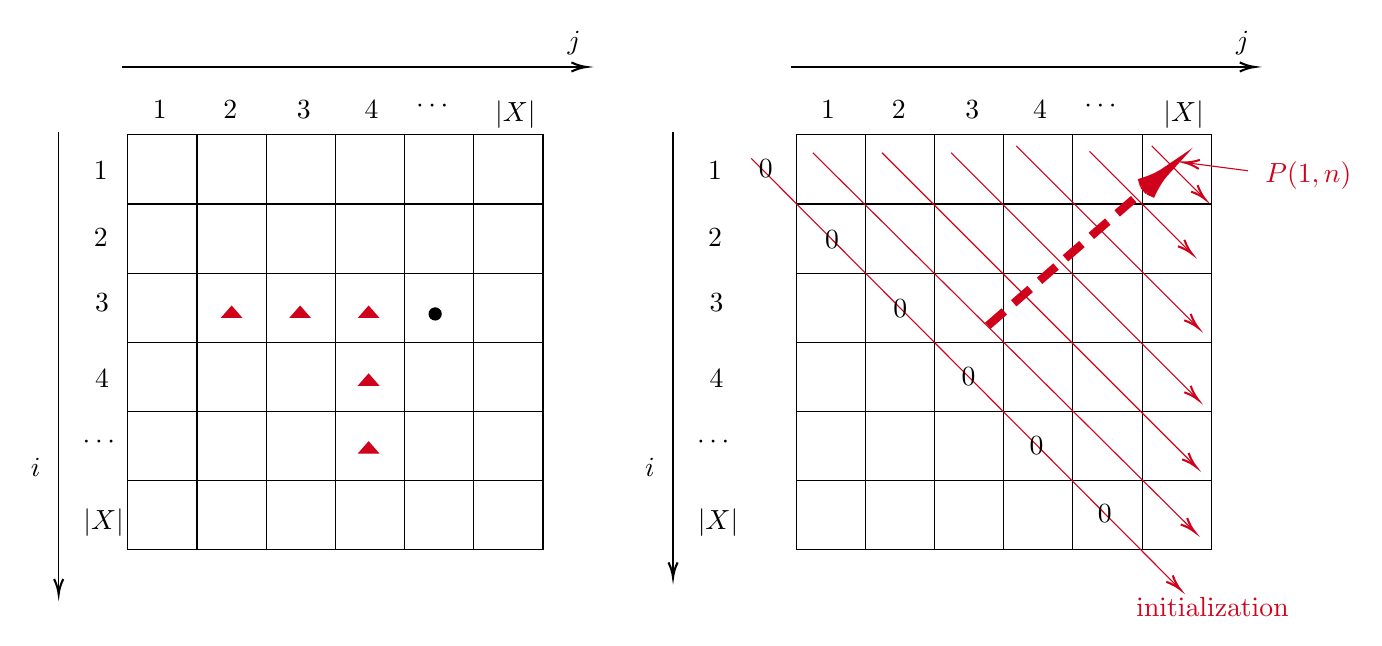
\begin{tikzpicture}[x=0.5pt,y=0.5pt,yscale=-1,xscale=1]
%uncomment if require: \path (0,447); %set diagram left start at 0, and has height of 447

%Shape: Grid [id:dp9095284515127875] 
\draw  [draw opacity=0] (87,90) -- (387,90) -- (387,390) -- (87,390) -- cycle ; \draw   (137,90) -- (137,390)(187,90) -- (187,390)(237,90) -- (237,390)(287,90) -- (287,390)(337,90) -- (337,390) ; \draw   (87,140) -- (387,140)(87,190) -- (387,190)(87,240) -- (387,240)(87,290) -- (387,290)(87,340) -- (387,340) ; \draw   (87,90) -- (387,90) -- (387,390) -- (87,390) -- cycle ;
%Straight Lines [id:da5347307434268296] 
\draw    (37,88) -- (37,420) ;
\draw [shift={(37,422)}, rotate = 270] [color={rgb, 255:red, 0; green, 0; blue, 0 }  ][line width=0.75]    (10.93,-3.29) .. controls (6.95,-1.4) and (3.31,-0.3) .. (0,0) .. controls (3.31,0.3) and (6.95,1.4) .. (10.93,3.29)   ;
%Straight Lines [id:da4989887299865372] 
\draw    (83,41) -- (416.5,41) ;
\draw [shift={(418.5,41)}, rotate = 180] [color={rgb, 255:red, 0; green, 0; blue, 0 }  ][line width=0.75]    (10.93,-3.29) .. controls (6.95,-1.4) and (3.31,-0.3) .. (0,0) .. controls (3.31,0.3) and (6.95,1.4) .. (10.93,3.29)   ;
%Flowchart: Connector [id:dp07878936208838816] 
\draw  [fill={rgb, 255:red, 0; green, 0; blue, 0 }  ,fill opacity=1 ] (305,217.9) .. controls (305.87,215.65) and (308.4,214.52) .. (310.66,215.39) .. controls (312.91,216.26) and (314.04,218.79) .. (313.17,221.05) .. controls (312.3,223.3) and (309.77,224.43) .. (307.51,223.56) .. controls (305.26,222.69) and (304.13,220.16) .. (305,217.9) -- cycle ;
%Shape: Triangle [id:dp6109876057002935] 
\draw  [color={rgb, 255:red, 208; green, 2; blue, 27 }  ,draw opacity=1 ][fill={rgb, 255:red, 208; green, 2; blue, 27 }  ,fill opacity=1 ] (261,214) -- (268,222) -- (254,222) -- cycle ;
%Shape: Triangle [id:dp003677095504452388] 
\draw  [color={rgb, 255:red, 208; green, 2; blue, 27 }  ,draw opacity=1 ][fill={rgb, 255:red, 208; green, 2; blue, 27 }  ,fill opacity=1 ] (211.5,214) -- (218.5,222) -- (204.5,222) -- cycle ;
%Shape: Triangle [id:dp543232883301439] 
\draw  [color={rgb, 255:red, 208; green, 2; blue, 27 }  ,draw opacity=1 ][fill={rgb, 255:red, 208; green, 2; blue, 27 }  ,fill opacity=1 ] (162,214) -- (169,222) -- (155,222) -- cycle ;
%Shape: Triangle [id:dp29900180690969524] 
\draw  [color={rgb, 255:red, 208; green, 2; blue, 27 }  ,draw opacity=1 ][fill={rgb, 255:red, 208; green, 2; blue, 27 }  ,fill opacity=1 ] (261,263) -- (268,271) -- (254,271) -- cycle ;
%Shape: Triangle [id:dp5517868734647194] 
\draw  [color={rgb, 255:red, 208; green, 2; blue, 27 }  ,draw opacity=1 ][fill={rgb, 255:red, 208; green, 2; blue, 27 }  ,fill opacity=1 ] (261,312) -- (268,320) -- (254,320) -- cycle ;
%Shape: Grid [id:dp8676217076414684] 
\draw  [draw opacity=0] (570,90) -- (870,90) -- (870,390) -- (570,390) -- cycle ; \draw   (620,90) -- (620,390)(670,90) -- (670,390)(720,90) -- (720,390)(770,90) -- (770,390)(820,90) -- (820,390) ; \draw   (570,140) -- (870,140)(570,190) -- (870,190)(570,240) -- (870,240)(570,290) -- (870,290)(570,340) -- (870,340) ; \draw   (570,90) -- (870,90) -- (870,390) -- (570,390) -- cycle ;
%Straight Lines [id:da23917339503157053] 
\draw    (481,88) -- (481,408) ;
\draw [shift={(481,410)}, rotate = 270] [color={rgb, 255:red, 0; green, 0; blue, 0 }  ][line width=0.75]    (10.93,-3.29) .. controls (6.95,-1.4) and (3.31,-0.3) .. (0,0) .. controls (3.31,0.3) and (6.95,1.4) .. (10.93,3.29)   ;
%Straight Lines [id:da1200250503088851] 
\draw    (566,41) -- (899.5,41) ;
\draw [shift={(901.5,41)}, rotate = 180] [color={rgb, 255:red, 0; green, 0; blue, 0 }  ][line width=0.75]    (10.93,-3.29) .. controls (6.95,-1.4) and (3.31,-0.3) .. (0,0) .. controls (3.31,0.3) and (6.95,1.4) .. (10.93,3.29)   ;
%Straight Lines [id:da5849775638339646] 
\draw [color={rgb, 255:red, 208; green, 2; blue, 27 }  ,draw opacity=1 ]   (896.5,116) -- (852.48,110.26) ;
\draw [shift={(850.5,110)}, rotate = 367.43] [color={rgb, 255:red, 208; green, 2; blue, 27 }  ,draw opacity=1 ][line width=0.75]    (10.93,-3.29) .. controls (6.95,-1.4) and (3.31,-0.3) .. (0,0) .. controls (3.31,0.3) and (6.95,1.4) .. (10.93,3.29)   ;
%Straight Lines [id:da7158674315801672] 
\draw [color={rgb, 255:red, 208; green, 2; blue, 27 }  ,draw opacity=1 ]   (537.5,107) -- (846.09,417.08) ;
\draw [shift={(847.5,418.5)}, rotate = 225.14] [color={rgb, 255:red, 208; green, 2; blue, 27 }  ,draw opacity=1 ][line width=0.75]    (10.93,-3.29) .. controls (6.95,-1.4) and (3.31,-0.3) .. (0,0) .. controls (3.31,0.3) and (6.95,1.4) .. (10.93,3.29)   ;
%Straight Lines [id:da06318163354731099] 
\draw [color={rgb, 255:red, 208; green, 2; blue, 27 }  ,draw opacity=1 ]   (582,103) -- (856.58,375.59) ;
\draw [shift={(858,377)}, rotate = 224.79] [color={rgb, 255:red, 208; green, 2; blue, 27 }  ,draw opacity=1 ][line width=0.75]    (10.93,-3.29) .. controls (6.95,-1.4) and (3.31,-0.3) .. (0,0) .. controls (3.31,0.3) and (6.95,1.4) .. (10.93,3.29)   ;
%Straight Lines [id:da7422545951430948] 
\draw [color={rgb, 255:red, 208; green, 2; blue, 27 }  ,draw opacity=1 ]   (632,103) -- (857.59,328.59) ;
\draw [shift={(859,330)}, rotate = 225] [color={rgb, 255:red, 208; green, 2; blue, 27 }  ,draw opacity=1 ][line width=0.75]    (10.93,-3.29) .. controls (6.95,-1.4) and (3.31,-0.3) .. (0,0) .. controls (3.31,0.3) and (6.95,1.4) .. (10.93,3.29)   ;
%Straight Lines [id:da6389984033381221] 
\draw [color={rgb, 255:red, 208; green, 2; blue, 27 }  ,draw opacity=1 ]   (682,103) -- (859.09,280.09) ;
\draw [shift={(860.5,281.5)}, rotate = 225] [color={rgb, 255:red, 208; green, 2; blue, 27 }  ,draw opacity=1 ][line width=0.75]    (10.93,-3.29) .. controls (6.95,-1.4) and (3.31,-0.3) .. (0,0) .. controls (3.31,0.3) and (6.95,1.4) .. (10.93,3.29)   ;
%Straight Lines [id:da7613617756284687] 
\draw [color={rgb, 255:red, 208; green, 2; blue, 27 }  ,draw opacity=1 ]   (729,98) -- (859.09,228.09) ;
\draw [shift={(860.5,229.5)}, rotate = 225] [color={rgb, 255:red, 208; green, 2; blue, 27 }  ,draw opacity=1 ][line width=0.75]    (10.93,-3.29) .. controls (6.95,-1.4) and (3.31,-0.3) .. (0,0) .. controls (3.31,0.3) and (6.95,1.4) .. (10.93,3.29)   ;
%Straight Lines [id:da7035765059521567] 
\draw [color={rgb, 255:red, 208; green, 2; blue, 27 }  ,draw opacity=1 ]   (782,102) -- (854.59,174.59) ;
\draw [shift={(856,176)}, rotate = 225] [color={rgb, 255:red, 208; green, 2; blue, 27 }  ,draw opacity=1 ][line width=0.75]    (10.93,-3.29) .. controls (6.95,-1.4) and (3.31,-0.3) .. (0,0) .. controls (3.31,0.3) and (6.95,1.4) .. (10.93,3.29)   ;
%Straight Lines [id:da156242521236438] 
\draw [color={rgb, 255:red, 208; green, 2; blue, 27 }  ,draw opacity=1 ]   (827,98) -- (864.09,135.09) ;
\draw [shift={(865.5,136.5)}, rotate = 225] [color={rgb, 255:red, 208; green, 2; blue, 27 }  ,draw opacity=1 ][line width=0.75]    (10.93,-3.29) .. controls (6.95,-1.4) and (3.31,-0.3) .. (0,0) .. controls (3.31,0.3) and (6.95,1.4) .. (10.93,3.29)   ;
%Straight Lines [id:da421849353700268] 
\draw [color={rgb, 255:red, 208; green, 2; blue, 27 }  ,draw opacity=1 ][line width=3]  [dash pattern={on 7.88pt off 4.5pt}]  (708.5,228) -- (833.72,119.28) ;
\draw [shift={(837.5,116)}, rotate = 499.03] [color={rgb, 255:red, 208; green, 2; blue, 27 }  ,draw opacity=1 ][line width=3]    (20.77,-6.25) .. controls (13.2,-2.65) and (6.28,-0.57) .. (0,0) .. controls (6.28,0.57) and (13.2,2.66) .. (20.77,6.25)   ;

% Text Node
\draw (68,103) node [anchor=north west][inner sep=0.75pt]   [align=left] {$ $};
% Text Node
\draw (60.5,107.38) node [anchor=north west][inner sep=0.75pt]   [align=left] {$\displaystyle 1$};
% Text Node
\draw (52.5,306.14) node [anchor=north west][inner sep=0.75pt]   [align=left] {$\displaystyle \cdots $};
% Text Node
\draw (15,322) node [anchor=north west][inner sep=0.75pt]   [align=left] {$\displaystyle i$};
% Text Node
\draw (403,13) node [anchor=north west][inner sep=0.75pt]   [align=left] {$\displaystyle j$};
% Text Node
\draw (293.4,63.44) node [anchor=north west][inner sep=0.75pt]   [align=left] {$\displaystyle \cdots $};
% Text Node
\draw (60.5,155.76) node [anchor=north west][inner sep=0.75pt]   [align=left] {$\displaystyle 2$};
% Text Node
\draw (103.1,63.44) node [anchor=north west][inner sep=0.75pt]   [align=left] {$\displaystyle 1$};
% Text Node
\draw (154.2,63.44) node [anchor=north west][inner sep=0.75pt]   [align=left] {$\displaystyle 2$};
% Text Node
\draw (350.5,63.44) node [anchor=north west][inner sep=0.75pt]   [align=left] {$\displaystyle | X|$};
% Text Node
\draw (207.3,63.44) node [anchor=north west][inner sep=0.75pt]   [align=left] {$\displaystyle 3$};
% Text Node
\draw (53,358.5) node [anchor=north west][inner sep=0.75pt]   [align=left] {$\displaystyle | X|$};
% Text Node
\draw (61.5,202.76) node [anchor=north west][inner sep=0.75pt]   [align=left] {$\displaystyle 3$};
% Text Node
\draw (61.5,257.76) node [anchor=north west][inner sep=0.75pt]   [align=left] {$\displaystyle 4$};
% Text Node
\draw (256.3,63.44) node [anchor=north west][inner sep=0.75pt]   [align=left] {$\displaystyle 4$};
% Text Node
\draw (512,103) node [anchor=north west][inner sep=0.75pt]   [align=left] {$ $};
% Text Node
\draw (504.5,107.38) node [anchor=north west][inner sep=0.75pt]   [align=left] {$\displaystyle 1$};
% Text Node
\draw (496.5,306.14) node [anchor=north west][inner sep=0.75pt]   [align=left] {$\displaystyle \cdots $};
% Text Node
\draw (459,322) node [anchor=north west][inner sep=0.75pt]   [align=left] {$\displaystyle i$};
% Text Node
\draw (886,13) node [anchor=north west][inner sep=0.75pt]   [align=left] {$\displaystyle j$};
% Text Node
\draw (776.4,63.44) node [anchor=north west][inner sep=0.75pt]   [align=left] {$\displaystyle \cdots $};
% Text Node
\draw (504.5,155.76) node [anchor=north west][inner sep=0.75pt]   [align=left] {$\displaystyle 2$};
% Text Node
\draw (586.1,63.44) node [anchor=north west][inner sep=0.75pt]   [align=left] {$\displaystyle 1$};
% Text Node
\draw (637.2,63.44) node [anchor=north west][inner sep=0.75pt]   [align=left] {$\displaystyle 2$};
% Text Node
\draw (833.5,63.44) node [anchor=north west][inner sep=0.75pt]   [align=left] {$\displaystyle | X|$};
% Text Node
\draw (690.3,63.44) node [anchor=north west][inner sep=0.75pt]   [align=left] {$\displaystyle 3$};
% Text Node
\draw (907.2,107.44) node [anchor=north west][inner sep=0.75pt]   [align=left] {$\displaystyle \textcolor[rgb]{0.82,0.01,0.11}{P}\textcolor[rgb]{0.82,0.01,0.11}{(}\textcolor[rgb]{0.82,0.01,0.11}{1,n}\textcolor[rgb]{0.82,0.01,0.11}{)}$};
% Text Node
\draw (497,358.5) node [anchor=north west][inner sep=0.75pt]   [align=left] {$\displaystyle | X|$};
% Text Node
\draw (505.5,202.76) node [anchor=north west][inner sep=0.75pt]   [align=left] {$\displaystyle 3$};
% Text Node
\draw (505.5,257.76) node [anchor=north west][inner sep=0.75pt]   [align=left] {$\displaystyle 4$};
% Text Node
\draw (739.3,63.44) node [anchor=north west][inner sep=0.75pt]   [align=left] {$\displaystyle 4$};
% Text Node
\draw (589.1,157.44) node [anchor=north west][inner sep=0.75pt]   [align=left] {$\displaystyle 0$};
% Text Node
\draw (638.35,206.94) node [anchor=north west][inner sep=0.75pt]   [align=left] {$\displaystyle 0$};
% Text Node
\draw (687.6,256.44) node [anchor=north west][inner sep=0.75pt]   [align=left] {$\displaystyle 0$};
% Text Node
\draw (736.85,305.94) node [anchor=north west][inner sep=0.75pt]   [align=left] {$\displaystyle 0$};
% Text Node
\draw (786.1,355.44) node [anchor=north west][inner sep=0.75pt]   [align=left] {$\displaystyle 0$};
% Text Node
\draw (814,422) node [anchor=north west][inner sep=0.75pt]   [align=left] {\textcolor[rgb]{0.82,0.01,0.11}{initialization}};
% Text Node
\draw (541.1,106.44) node [anchor=north west][inner sep=0.75pt]   [align=left] {$\displaystyle 0$};


\end{tikzpicture}

}
\caption{The dynamic programming table.}
\label{fig:table}
\end{figure}


\begin{minipage}{0.8\textwidth}
	\aaA {9}{Algorithm edit-distance~(two strings $X$, $Y$)}\xxx
	\aab {$F(0,j) = j$, for any $0 \le j \le |Y|$}\xxx
	\aab {$F(i,0) = i$, for any $0 \le i \le |X|$}\xxx
	\aaB {4}{for $i = 1 \to |X|$}\xxx
	\aaC {2}{for $j = 1 \to |Y|$}\xxx
	\aad {$F(i,j) = \min\{F(i-1,j-1) + \delta(X[i] \neq Y[j]), F(i-1,j) + 1, F(i,j-1) + 1\}$;}\xxx
	\aac {end for;}\xxx
	\aab {end for;}\xxx
	\aab {report: $F(|X|,|Y|) = d(X,Y)$;}\xxx
	\aaa {end algorithm;}\xxx
\end{minipage}

\subsection*{Transforming into Shortest Path Problem}

Another way to solve the edit distance problem is to transform it into a shortest-path problem.
See Figure~\ref{fig:graph}.
We build a graph with $(|X| + 1)(|Y| + 1)$ vertices, $v_{ij}$, $0\le 0 \le |X|$ and $0\le j \le |Y|$. 
(Imagine placing a vertex in each entry of above DP table.)
There are three in-edges for vertex $v_{ij}$, when $i\ge 1$ and $j \ge 1$, corresponding to
the 3 cases of the recursion. 
All vertical edges have edge length of 1;
all horizontal edges have edge length of 1;
all diagonal edges have edge length of either 1 or 0: 
if $X[i] \neq Y[j]$ then the edge $(v_{i-1,j-1}, v_{ij})$ has a length of 1,
and otherwise this edge has a length of 0.

\begin{figure}[h]
\centering{

\tikzset{every picture/.style={line width=0.75pt}} %set default line width to 0.75pt        

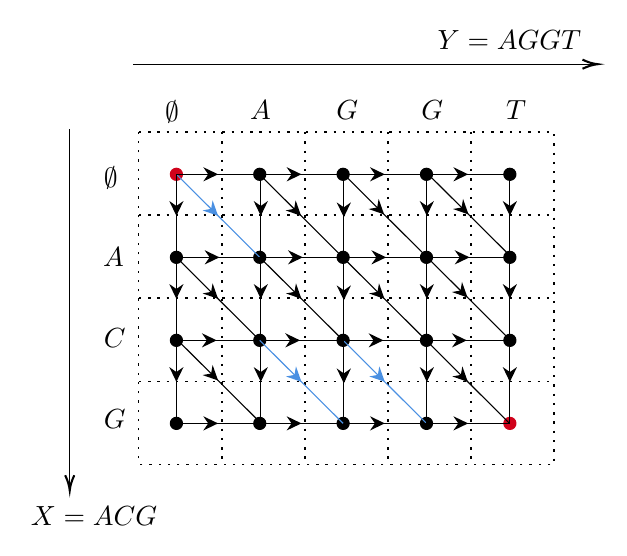
\begin{tikzpicture}[x=0.5pt,y=0.5pt,yscale=-1,xscale=1]
%uncomment if require: \path (0,392); %set diagram left start at 0, and has height of 392

%Shape: Grid [id:dp9095284515127875] 
\draw  [draw opacity=0][dash pattern={on 0.84pt off 2.51pt}] (87,90) -- (387,90) -- (387,330) -- (87,330) -- cycle ; \draw  [dash pattern={on 0.84pt off 2.51pt}] (147,90) -- (147,330)(207,90) -- (207,330)(267,90) -- (267,330)(327,90) -- (327,330) ; \draw  [dash pattern={on 0.84pt off 2.51pt}] (87,150) -- (387,150)(87,210) -- (387,210)(87,270) -- (387,270) ; \draw  [dash pattern={on 0.84pt off 2.51pt}] (87,90) -- (387,90) -- (387,330) -- (87,330) -- cycle ;
%Straight Lines [id:da5347307434268296] 
\draw    (37,88) -- (37,347) ;
\draw [shift={(37,349)}, rotate = 270] [color={rgb, 255:red, 0; green, 0; blue, 0 }  ][line width=0.75]    (10.93,-3.29) .. controls (6.95,-1.4) and (3.31,-0.3) .. (0,0) .. controls (3.31,0.3) and (6.95,1.4) .. (10.93,3.29)   ;
%Straight Lines [id:da4989887299865372] 
\draw    (83,41) -- (416.5,41) ;
\draw [shift={(418.5,41)}, rotate = 180] [color={rgb, 255:red, 0; green, 0; blue, 0 }  ][line width=0.75]    (10.93,-3.29) .. controls (6.95,-1.4) and (3.31,-0.3) .. (0,0) .. controls (3.31,0.3) and (6.95,1.4) .. (10.93,3.29)   ;
%Flowchart: Connector [id:dp7892032191057772] 
\draw  [color={rgb, 255:red, 208; green, 2; blue, 27 }  ,draw opacity=1 ][fill={rgb, 255:red, 208; green, 2; blue, 27 }  ,fill opacity=1 ] (110,119) .. controls (110.87,116.74) and (113.4,115.62) .. (115.66,116.49) .. controls (117.91,117.36) and (119.04,119.89) .. (118.17,122.15) .. controls (117.3,124.4) and (114.77,125.53) .. (112.51,124.66) .. controls (110.26,123.79) and (109.13,121.26) .. (110,119) -- cycle ;
%Flowchart: Connector [id:dp49117478027570705] 
\draw  [fill={rgb, 255:red, 0; green, 0; blue, 0 }  ,fill opacity=1 ] (170.25,119) .. controls (171.11,116.74) and (173.65,115.62) .. (175.9,116.49) .. controls (178.16,117.36) and (179.28,119.89) .. (178.41,122.15) .. controls (177.54,124.4) and (175.01,125.53) .. (172.76,124.66) .. controls (170.5,123.79) and (169.38,121.26) .. (170.25,119) -- cycle ;
%Flowchart: Connector [id:dp26507656226704346] 
\draw  [fill={rgb, 255:red, 0; green, 0; blue, 0 }  ,fill opacity=1 ] (230.49,119) .. controls (231.36,116.74) and (233.89,115.62) .. (236.15,116.49) .. controls (238.4,117.36) and (239.53,119.89) .. (238.66,122.15) .. controls (237.79,124.4) and (235.26,125.53) .. (233,124.66) .. controls (230.75,123.79) and (229.62,121.26) .. (230.49,119) -- cycle ;
%Flowchart: Connector [id:dp5898833817102163] 
\draw  [fill={rgb, 255:red, 0; green, 0; blue, 0 }  ,fill opacity=1 ] (290.74,119) .. controls (291.6,116.74) and (294.14,115.62) .. (296.39,116.49) .. controls (298.65,117.36) and (299.77,119.89) .. (298.9,122.15) .. controls (298.03,124.4) and (295.5,125.53) .. (293.25,124.66) .. controls (290.99,123.79) and (289.87,121.26) .. (290.74,119) -- cycle ;
%Flowchart: Connector [id:dp6978330041031003] 
\draw  [fill={rgb, 255:red, 0; green, 0; blue, 0 }  ,fill opacity=1 ] (351,119) .. controls (351.87,116.74) and (354.4,115.62) .. (356.66,116.49) .. controls (358.91,117.36) and (360.04,119.89) .. (359.17,122.15) .. controls (358.3,124.4) and (355.77,125.53) .. (353.51,124.66) .. controls (351.26,123.79) and (350.13,121.26) .. (351,119) -- cycle ;
%Flowchart: Connector [id:dp8787867823869434] 
\draw  [fill={rgb, 255:red, 0; green, 0; blue, 0 }  ,fill opacity=1 ] (110,179) .. controls (110.87,176.74) and (113.4,175.62) .. (115.66,176.48) .. controls (117.91,177.35) and (119.04,179.89) .. (118.17,182.14) .. controls (117.3,184.4) and (114.77,185.52) .. (112.51,184.65) .. controls (110.26,183.78) and (109.13,181.25) .. (110,179) -- cycle ;
%Flowchart: Connector [id:dp0009714153628327393] 
\draw  [fill={rgb, 255:red, 0; green, 0; blue, 0 }  ,fill opacity=1 ] (170.25,179) .. controls (171.11,176.74) and (173.65,175.62) .. (175.9,176.48) .. controls (178.16,177.35) and (179.28,179.89) .. (178.41,182.14) .. controls (177.54,184.4) and (175.01,185.52) .. (172.76,184.65) .. controls (170.5,183.78) and (169.38,181.25) .. (170.25,179) -- cycle ;
%Flowchart: Connector [id:dp9618763382927992] 
\draw  [fill={rgb, 255:red, 0; green, 0; blue, 0 }  ,fill opacity=1 ] (230.49,179) .. controls (231.36,176.74) and (233.89,175.62) .. (236.15,176.48) .. controls (238.4,177.35) and (239.53,179.89) .. (238.66,182.14) .. controls (237.79,184.4) and (235.26,185.52) .. (233,184.65) .. controls (230.75,183.78) and (229.62,181.25) .. (230.49,179) -- cycle ;
%Flowchart: Connector [id:dp9943373545221997] 
\draw  [fill={rgb, 255:red, 0; green, 0; blue, 0 }  ,fill opacity=1 ] (290.74,179) .. controls (291.6,176.74) and (294.14,175.62) .. (296.39,176.48) .. controls (298.65,177.35) and (299.77,179.89) .. (298.9,182.14) .. controls (298.03,184.4) and (295.5,185.52) .. (293.25,184.65) .. controls (290.99,183.78) and (289.87,181.25) .. (290.74,179) -- cycle ;
%Flowchart: Connector [id:dp482699380394507] 
\draw  [fill={rgb, 255:red, 0; green, 0; blue, 0 }  ,fill opacity=1 ] (351,179) .. controls (351.87,176.74) and (354.4,175.62) .. (356.66,176.48) .. controls (358.91,177.35) and (360.04,179.89) .. (359.17,182.14) .. controls (358.3,184.4) and (355.77,185.52) .. (353.51,184.65) .. controls (351.26,183.78) and (350.13,181.25) .. (351,179) -- cycle ;

%Flowchart: Connector [id:dp7087606993451726] 
\draw  [fill={rgb, 255:red, 0; green, 0; blue, 0 }  ,fill opacity=1 ] (110,238.99) .. controls (110.87,236.73) and (113.4,235.61) .. (115.66,236.48) .. controls (117.91,237.35) and (119.04,239.88) .. (118.17,242.14) .. controls (117.3,244.39) and (114.77,245.52) .. (112.51,244.65) .. controls (110.26,243.78) and (109.13,241.25) .. (110,238.99) -- cycle ;
%Flowchart: Connector [id:dp38414449021330055] 
\draw  [fill={rgb, 255:red, 0; green, 0; blue, 0 }  ,fill opacity=1 ] (170.25,238.99) .. controls (171.11,236.73) and (173.65,235.61) .. (175.9,236.48) .. controls (178.16,237.35) and (179.28,239.88) .. (178.41,242.14) .. controls (177.54,244.39) and (175.01,245.52) .. (172.76,244.65) .. controls (170.5,243.78) and (169.38,241.25) .. (170.25,238.99) -- cycle ;
%Flowchart: Connector [id:dp2499479633678482] 
\draw  [fill={rgb, 255:red, 0; green, 0; blue, 0 }  ,fill opacity=1 ] (230.49,238.99) .. controls (231.36,236.73) and (233.89,235.61) .. (236.15,236.48) .. controls (238.4,237.35) and (239.53,239.88) .. (238.66,242.14) .. controls (237.79,244.39) and (235.26,245.52) .. (233,244.65) .. controls (230.75,243.78) and (229.62,241.25) .. (230.49,238.99) -- cycle ;
%Flowchart: Connector [id:dp3150236979186747] 
\draw  [fill={rgb, 255:red, 0; green, 0; blue, 0 }  ,fill opacity=1 ] (290.74,238.99) .. controls (291.6,236.73) and (294.14,235.61) .. (296.39,236.48) .. controls (298.65,237.35) and (299.77,239.88) .. (298.9,242.14) .. controls (298.03,244.39) and (295.5,245.52) .. (293.25,244.65) .. controls (290.99,243.78) and (289.87,241.25) .. (290.74,238.99) -- cycle ;
%Flowchart: Connector [id:dp5548250717430041] 
\draw  [fill={rgb, 255:red, 0; green, 0; blue, 0 }  ,fill opacity=1 ] (351,238.99) .. controls (351.87,236.73) and (354.4,235.61) .. (356.66,236.48) .. controls (358.91,237.35) and (360.04,239.88) .. (359.17,242.14) .. controls (358.3,244.39) and (355.77,245.52) .. (353.51,244.65) .. controls (351.26,243.78) and (350.13,241.25) .. (351,238.99) -- cycle ;

%Flowchart: Connector [id:dp6724053862379229] 
\draw  [fill={rgb, 255:red, 0; green, 0; blue, 0 }  ,fill opacity=1 ] (110,299) .. controls (110.87,296.74) and (113.4,295.62) .. (115.66,296.49) .. controls (117.91,297.36) and (119.04,299.89) .. (118.17,302.15) .. controls (117.3,304.4) and (114.77,305.53) .. (112.51,304.66) .. controls (110.26,303.79) and (109.13,301.26) .. (110,299) -- cycle ;
%Flowchart: Connector [id:dp809285050914335] 
\draw  [fill={rgb, 255:red, 0; green, 0; blue, 0 }  ,fill opacity=1 ] (170.25,299) .. controls (171.11,296.74) and (173.65,295.62) .. (175.9,296.49) .. controls (178.16,297.36) and (179.28,299.89) .. (178.41,302.15) .. controls (177.54,304.4) and (175.01,305.53) .. (172.76,304.66) .. controls (170.5,303.79) and (169.38,301.26) .. (170.25,299) -- cycle ;
%Flowchart: Connector [id:dp1943046479465117] 
\draw  [fill={rgb, 255:red, 0; green, 0; blue, 0 }  ,fill opacity=1 ] (230.49,299) .. controls (231.36,296.74) and (233.89,295.62) .. (236.15,296.49) .. controls (238.4,297.36) and (239.53,299.89) .. (238.66,302.15) .. controls (237.79,304.4) and (235.26,305.53) .. (233,304.66) .. controls (230.75,303.79) and (229.62,301.26) .. (230.49,299) -- cycle ;
%Flowchart: Connector [id:dp17706594266241393] 
\draw  [fill={rgb, 255:red, 0; green, 0; blue, 0 }  ,fill opacity=1 ] (290.74,299) .. controls (291.6,296.74) and (294.14,295.62) .. (296.39,296.49) .. controls (298.65,297.36) and (299.77,299.89) .. (298.9,302.15) .. controls (298.03,304.4) and (295.5,305.53) .. (293.25,304.66) .. controls (290.99,303.79) and (289.87,301.26) .. (290.74,299) -- cycle ;
%Flowchart: Connector [id:dp06123722582552604] 
\draw  [color={rgb, 255:red, 208; green, 2; blue, 27 }  ,draw opacity=1 ][fill={rgb, 255:red, 208; green, 2; blue, 27 }  ,fill opacity=1 ] (351,299) .. controls (351.87,296.74) and (354.4,295.62) .. (356.66,296.49) .. controls (358.91,297.36) and (360.04,299.89) .. (359.17,302.15) .. controls (358.3,304.4) and (355.77,305.53) .. (353.51,304.66) .. controls (351.26,303.79) and (350.13,301.26) .. (351,299) -- cycle ;
%Straight Lines [id:da3592419747103084] 
\draw [color={rgb, 255:red, 74; green, 144; blue, 226 }  ,draw opacity=1 ]   (114.08,120.57) -- (174.33,180.57) ;
\draw [shift={(144.21,150.57)}, rotate = 224.88] [fill={rgb, 255:red, 74; green, 144; blue, 226 }  ,fill opacity=1 ][line width=0.08]  [draw opacity=0] (10.72,-5.15) -- (0,0) -- (10.72,5.15) -- (7.12,0) -- cycle    ;
%Straight Lines [id:da11016791165620432] 
\draw    (174.33,180.57) -- (234.57,240.56) ;
\draw [shift={(204.45,210.57)}, rotate = 224.88] [fill={rgb, 255:red, 0; green, 0; blue, 0 }  ][line width=0.08]  [draw opacity=0] (10.72,-5.15) -- (0,0) -- (10.72,5.15) -- (7.12,0) -- cycle    ;
%Straight Lines [id:da861324040374141] 
\draw [color={rgb, 255:red, 74; green, 144; blue, 226 }  ,draw opacity=1 ]   (234.57,240.56) -- (294.82,300.56) ;
\draw [shift={(264.7,270.56)}, rotate = 224.88] [fill={rgb, 255:red, 74; green, 144; blue, 226 }  ,fill opacity=1 ][line width=0.08]  [draw opacity=0] (10.72,-5.15) -- (0,0) -- (10.72,5.15) -- (7.12,0) -- cycle    ;
%Straight Lines [id:da623241069163482] 
\draw    (114.08,120.57) -- (174.33,120.57) ;
\draw [shift={(144.21,120.57)}, rotate = 180] [fill={rgb, 255:red, 0; green, 0; blue, 0 }  ][line width=0.08]  [draw opacity=0] (10.72,-5.15) -- (0,0) -- (10.72,5.15) -- (7.12,0) -- cycle    ;
%Straight Lines [id:da6849986890026631] 
\draw    (174.33,120.57) -- (234.57,120.57) ;
\draw [shift={(204.45,120.57)}, rotate = 180] [fill={rgb, 255:red, 0; green, 0; blue, 0 }  ][line width=0.08]  [draw opacity=0] (10.72,-5.15) -- (0,0) -- (10.72,5.15) -- (7.12,0) -- cycle    ;
%Straight Lines [id:da041846349377336334] 
\draw    (234.57,120.57) -- (294.82,120.57) ;
\draw [shift={(264.7,120.57)}, rotate = 180] [fill={rgb, 255:red, 0; green, 0; blue, 0 }  ][line width=0.08]  [draw opacity=0] (10.72,-5.15) -- (0,0) -- (10.72,5.15) -- (7.12,0) -- cycle    ;
%Straight Lines [id:da39569790466634525] 
\draw    (294.82,120.57) -- (355.06,120.57) ;
\draw [shift={(324.94,120.57)}, rotate = 180] [fill={rgb, 255:red, 0; green, 0; blue, 0 }  ][line width=0.08]  [draw opacity=0] (10.72,-5.15) -- (0,0) -- (10.72,5.15) -- (7.12,0) -- cycle    ;
%Straight Lines [id:da03525501140121612] 
\draw    (115.08,180.57) -- (175.33,180.57) ;
\draw [shift={(145.21,180.57)}, rotate = 180] [fill={rgb, 255:red, 0; green, 0; blue, 0 }  ][line width=0.08]  [draw opacity=0] (10.72,-5.15) -- (0,0) -- (10.72,5.15) -- (7.12,0) -- cycle    ;
%Straight Lines [id:da5053376972804251] 
\draw    (175.33,180.57) -- (235.57,180.57) ;
\draw [shift={(205.45,180.57)}, rotate = 180] [fill={rgb, 255:red, 0; green, 0; blue, 0 }  ][line width=0.08]  [draw opacity=0] (10.72,-5.15) -- (0,0) -- (10.72,5.15) -- (7.12,0) -- cycle    ;
%Straight Lines [id:da9403450630282508] 
\draw    (235.57,180.57) -- (295.82,180.57) ;
\draw [shift={(265.7,180.57)}, rotate = 180] [fill={rgb, 255:red, 0; green, 0; blue, 0 }  ][line width=0.08]  [draw opacity=0] (10.72,-5.15) -- (0,0) -- (10.72,5.15) -- (7.12,0) -- cycle    ;
%Straight Lines [id:da8252476547397996] 
\draw    (295.82,180.57) -- (356.06,180.57) ;
\draw [shift={(325.94,180.57)}, rotate = 180] [fill={rgb, 255:red, 0; green, 0; blue, 0 }  ][line width=0.08]  [draw opacity=0] (10.72,-5.15) -- (0,0) -- (10.72,5.15) -- (7.12,0) -- cycle    ;
%Straight Lines [id:da20328228934926562] 
\draw    (113.08,240.57) -- (173.33,240.57) ;
\draw [shift={(143.21,240.57)}, rotate = 180] [fill={rgb, 255:red, 0; green, 0; blue, 0 }  ][line width=0.08]  [draw opacity=0] (10.72,-5.15) -- (0,0) -- (10.72,5.15) -- (7.12,0) -- cycle    ;
%Straight Lines [id:da18936177213663397] 
\draw    (173.33,240.57) -- (233.57,240.57) ;
\draw [shift={(203.45,240.57)}, rotate = 180] [fill={rgb, 255:red, 0; green, 0; blue, 0 }  ][line width=0.08]  [draw opacity=0] (10.72,-5.15) -- (0,0) -- (10.72,5.15) -- (7.12,0) -- cycle    ;
%Straight Lines [id:da5472813253116537] 
\draw    (233.57,240.57) -- (293.82,240.57) ;
\draw [shift={(263.7,240.57)}, rotate = 180] [fill={rgb, 255:red, 0; green, 0; blue, 0 }  ][line width=0.08]  [draw opacity=0] (10.72,-5.15) -- (0,0) -- (10.72,5.15) -- (7.12,0) -- cycle    ;
%Straight Lines [id:da18891264531279117] 
\draw    (293.82,240.57) -- (354.06,240.57) ;
\draw [shift={(323.94,240.57)}, rotate = 180] [fill={rgb, 255:red, 0; green, 0; blue, 0 }  ][line width=0.08]  [draw opacity=0] (10.72,-5.15) -- (0,0) -- (10.72,5.15) -- (7.12,0) -- cycle    ;
%Straight Lines [id:da39657569614796095] 
\draw    (114.08,300.57) -- (174.33,300.57) ;
\draw [shift={(144.21,300.57)}, rotate = 180] [fill={rgb, 255:red, 0; green, 0; blue, 0 }  ][line width=0.08]  [draw opacity=0] (10.72,-5.15) -- (0,0) -- (10.72,5.15) -- (7.12,0) -- cycle    ;
%Straight Lines [id:da3308363661164806] 
\draw    (174.33,300.57) -- (234.57,300.57) ;
\draw [shift={(204.45,300.57)}, rotate = 180] [fill={rgb, 255:red, 0; green, 0; blue, 0 }  ][line width=0.08]  [draw opacity=0] (10.72,-5.15) -- (0,0) -- (10.72,5.15) -- (7.12,0) -- cycle    ;
%Straight Lines [id:da899869033517725] 
\draw    (234.57,300.57) -- (294.82,300.57) ;
\draw [shift={(264.7,300.57)}, rotate = 180] [fill={rgb, 255:red, 0; green, 0; blue, 0 }  ][line width=0.08]  [draw opacity=0] (10.72,-5.15) -- (0,0) -- (10.72,5.15) -- (7.12,0) -- cycle    ;
%Straight Lines [id:da9491468552348531] 
\draw    (294.82,300.57) -- (355.06,300.57) ;
\draw [shift={(324.94,300.57)}, rotate = 180] [fill={rgb, 255:red, 0; green, 0; blue, 0 }  ][line width=0.08]  [draw opacity=0] (10.72,-5.15) -- (0,0) -- (10.72,5.15) -- (7.12,0) -- cycle    ;
%Straight Lines [id:da5447577825869346] 
\draw    (114.08,120.57) -- (114.08,180.57) ;
\draw [shift={(114.08,150.57)}, rotate = 270] [fill={rgb, 255:red, 0; green, 0; blue, 0 }  ][line width=0.08]  [draw opacity=0] (10.72,-5.15) -- (0,0) -- (10.72,5.15) -- (7.12,0) -- cycle    ;
%Straight Lines [id:da4468689576120938] 
\draw    (114.08,180.57) -- (114.08,240.56) ;
\draw [shift={(114.08,210.57)}, rotate = 270] [fill={rgb, 255:red, 0; green, 0; blue, 0 }  ][line width=0.08]  [draw opacity=0] (10.72,-5.15) -- (0,0) -- (10.72,5.15) -- (7.12,0) -- cycle    ;
%Straight Lines [id:da7974322408910806] 
\draw    (114.08,240.58) -- (114.08,300.57) ;
\draw [shift={(114.08,270.58)}, rotate = 270] [fill={rgb, 255:red, 0; green, 0; blue, 0 }  ][line width=0.08]  [draw opacity=0] (10.72,-5.15) -- (0,0) -- (10.72,5.15) -- (7.12,0) -- cycle    ;
%Straight Lines [id:da3348650527968928] 
\draw    (175.08,120.57) -- (175.08,180.57) ;
\draw [shift={(175.08,150.57)}, rotate = 270] [fill={rgb, 255:red, 0; green, 0; blue, 0 }  ][line width=0.08]  [draw opacity=0] (10.72,-5.15) -- (0,0) -- (10.72,5.15) -- (7.12,0) -- cycle    ;
%Straight Lines [id:da506734157691636] 
\draw    (175.08,180.57) -- (175.08,240.56) ;
\draw [shift={(175.08,210.57)}, rotate = 270] [fill={rgb, 255:red, 0; green, 0; blue, 0 }  ][line width=0.08]  [draw opacity=0] (10.72,-5.15) -- (0,0) -- (10.72,5.15) -- (7.12,0) -- cycle    ;
%Straight Lines [id:da5840193538092129] 
\draw    (175.08,240.58) -- (175.08,300.57) ;
\draw [shift={(175.08,270.58)}, rotate = 270] [fill={rgb, 255:red, 0; green, 0; blue, 0 }  ][line width=0.08]  [draw opacity=0] (10.72,-5.15) -- (0,0) -- (10.72,5.15) -- (7.12,0) -- cycle    ;
%Straight Lines [id:da23886443798971468] 
\draw    (235.08,121.57) -- (235.08,181.57) ;
\draw [shift={(235.08,151.57)}, rotate = 270] [fill={rgb, 255:red, 0; green, 0; blue, 0 }  ][line width=0.08]  [draw opacity=0] (10.72,-5.15) -- (0,0) -- (10.72,5.15) -- (7.12,0) -- cycle    ;
%Straight Lines [id:da7044289327291252] 
\draw    (235.08,181.57) -- (235.08,241.56) ;
\draw [shift={(235.08,211.57)}, rotate = 270] [fill={rgb, 255:red, 0; green, 0; blue, 0 }  ][line width=0.08]  [draw opacity=0] (10.72,-5.15) -- (0,0) -- (10.72,5.15) -- (7.12,0) -- cycle    ;
%Straight Lines [id:da3233842191612859] 
\draw    (235.08,241.58) -- (235.08,301.57) ;
\draw [shift={(235.08,271.58)}, rotate = 270] [fill={rgb, 255:red, 0; green, 0; blue, 0 }  ][line width=0.08]  [draw opacity=0] (10.72,-5.15) -- (0,0) -- (10.72,5.15) -- (7.12,0) -- cycle    ;
%Straight Lines [id:da2719581099277214] 
\draw    (295.08,120.57) -- (295.08,180.57) ;
\draw [shift={(295.08,150.57)}, rotate = 270] [fill={rgb, 255:red, 0; green, 0; blue, 0 }  ][line width=0.08]  [draw opacity=0] (10.72,-5.15) -- (0,0) -- (10.72,5.15) -- (7.12,0) -- cycle    ;
%Straight Lines [id:da7955951831524506] 
\draw    (295.08,180.57) -- (295.08,240.56) ;
\draw [shift={(295.08,210.57)}, rotate = 270] [fill={rgb, 255:red, 0; green, 0; blue, 0 }  ][line width=0.08]  [draw opacity=0] (10.72,-5.15) -- (0,0) -- (10.72,5.15) -- (7.12,0) -- cycle    ;
%Straight Lines [id:da5413316975942024] 
\draw    (295.08,240.58) -- (295.08,300.57) ;
\draw [shift={(295.08,270.58)}, rotate = 270] [fill={rgb, 255:red, 0; green, 0; blue, 0 }  ][line width=0.08]  [draw opacity=0] (10.72,-5.15) -- (0,0) -- (10.72,5.15) -- (7.12,0) -- cycle    ;
%Straight Lines [id:da528683157094314] 
\draw    (355.08,120.57) -- (355.08,180.57) ;
\draw [shift={(355.08,150.57)}, rotate = 270] [fill={rgb, 255:red, 0; green, 0; blue, 0 }  ][line width=0.08]  [draw opacity=0] (10.72,-5.15) -- (0,0) -- (10.72,5.15) -- (7.12,0) -- cycle    ;
%Straight Lines [id:da7884969890323227] 
\draw    (355.08,180.57) -- (355.08,240.56) ;
\draw [shift={(355.08,210.57)}, rotate = 270] [fill={rgb, 255:red, 0; green, 0; blue, 0 }  ][line width=0.08]  [draw opacity=0] (10.72,-5.15) -- (0,0) -- (10.72,5.15) -- (7.12,0) -- cycle    ;
%Straight Lines [id:da026306147500106514] 
\draw    (355.08,240.58) -- (355.08,300.57) ;
\draw [shift={(355.08,270.58)}, rotate = 270] [fill={rgb, 255:red, 0; green, 0; blue, 0 }  ][line width=0.08]  [draw opacity=0] (10.72,-5.15) -- (0,0) -- (10.72,5.15) -- (7.12,0) -- cycle    ;
%Straight Lines [id:da5304148083854859] 
\draw    (174.08,120.57) -- (234.33,180.57) ;
\draw [shift={(204.21,150.57)}, rotate = 224.88] [fill={rgb, 255:red, 0; green, 0; blue, 0 }  ][line width=0.08]  [draw opacity=0] (10.72,-5.15) -- (0,0) -- (10.72,5.15) -- (7.12,0) -- cycle    ;
%Straight Lines [id:da10387619856914898] 
\draw    (234.33,180.57) -- (294.57,240.56) ;
\draw [shift={(264.45,210.57)}, rotate = 224.88] [fill={rgb, 255:red, 0; green, 0; blue, 0 }  ][line width=0.08]  [draw opacity=0] (10.72,-5.15) -- (0,0) -- (10.72,5.15) -- (7.12,0) -- cycle    ;
%Straight Lines [id:da6684466112396508] 
\draw    (294.57,240.56) -- (354.82,300.56) ;
\draw [shift={(324.7,270.56)}, rotate = 224.88] [fill={rgb, 255:red, 0; green, 0; blue, 0 }  ][line width=0.08]  [draw opacity=0] (10.72,-5.15) -- (0,0) -- (10.72,5.15) -- (7.12,0) -- cycle    ;
%Straight Lines [id:da3445451700183738] 
\draw    (234.08,119.57) -- (294.33,179.57) ;
\draw [shift={(264.21,149.57)}, rotate = 224.88] [fill={rgb, 255:red, 0; green, 0; blue, 0 }  ][line width=0.08]  [draw opacity=0] (10.72,-5.15) -- (0,0) -- (10.72,5.15) -- (7.12,0) -- cycle    ;
%Straight Lines [id:da9388081629332891] 
\draw    (294.33,179.57) -- (354.57,239.56) ;
\draw [shift={(324.45,209.57)}, rotate = 224.88] [fill={rgb, 255:red, 0; green, 0; blue, 0 }  ][line width=0.08]  [draw opacity=0] (10.72,-5.15) -- (0,0) -- (10.72,5.15) -- (7.12,0) -- cycle    ;
%Straight Lines [id:da5665052547166216] 
\draw    (295.08,119.57) -- (355.33,179.57) ;
\draw [shift={(325.21,149.57)}, rotate = 224.88] [fill={rgb, 255:red, 0; green, 0; blue, 0 }  ][line width=0.08]  [draw opacity=0] (10.72,-5.15) -- (0,0) -- (10.72,5.15) -- (7.12,0) -- cycle    ;
%Straight Lines [id:da5547716631608589] 
\draw    (114.08,180.57) -- (174.33,240.57) ;
\draw [shift={(144.21,210.57)}, rotate = 224.88] [fill={rgb, 255:red, 0; green, 0; blue, 0 }  ][line width=0.08]  [draw opacity=0] (10.72,-5.15) -- (0,0) -- (10.72,5.15) -- (7.12,0) -- cycle    ;
%Straight Lines [id:da44797690158878345] 
\draw [color={rgb, 255:red, 74; green, 144; blue, 226 }  ,draw opacity=1 ]   (174.33,240.57) -- (234.57,300.56) ;
\draw [shift={(204.45,270.57)}, rotate = 224.88] [fill={rgb, 255:red, 74; green, 144; blue, 226 }  ,fill opacity=1 ][line width=0.08]  [draw opacity=0] (10.72,-5.15) -- (0,0) -- (10.72,5.15) -- (7.12,0) -- cycle    ;
%Straight Lines [id:da4158633112708935] 
\draw    (114.08,239.57) -- (174.33,299.57) ;
\draw [shift={(144.21,269.57)}, rotate = 224.88] [fill={rgb, 255:red, 0; green, 0; blue, 0 }  ][line width=0.08]  [draw opacity=0] (10.72,-5.15) -- (0,0) -- (10.72,5.15) -- (7.12,0) -- cycle    ;

% Text Node
\draw (68,103) node [anchor=north west][inner sep=0.75pt]   [align=left] {$ $};
% Text Node
\draw (59.25,171.5) node [anchor=north west][inner sep=0.75pt]   [align=left] {$\displaystyle A$};
% Text Node
\draw (59.75,230) node [anchor=north west][inner sep=0.75pt]   [align=left] {$\displaystyle C$};
% Text Node
\draw (7,359) node [anchor=north west][inner sep=0.75pt]   [align=left] {$\displaystyle X=ACG$};
% Text Node
\draw (301,15) node [anchor=north west][inner sep=0.75pt]   [align=left] {$\displaystyle Y=AGGT$};
% Text Node
\draw (104,65.44) node [anchor=north west][inner sep=0.75pt]   [align=left] {$\displaystyle \emptyset $};
% Text Node
\draw (289.14,65.44) node [anchor=north west][inner sep=0.75pt]   [align=left] {$\displaystyle G$};
% Text Node
\draw (59.75,113) node [anchor=north west][inner sep=0.75pt]   [align=left] {$\displaystyle \emptyset $};
% Text Node
\draw (59.75,288.5) node [anchor=north west][inner sep=0.75pt]   [align=left] {$\displaystyle G$};
% Text Node
\draw (165.38,65.44) node [anchor=north west][inner sep=0.75pt]   [align=left] {$\displaystyle A$};
% Text Node
\draw (227.76,65.44) node [anchor=north west][inner sep=0.75pt]   [align=left] {$\displaystyle G$};
% Text Node
\draw (350.5,65.44) node [anchor=north west][inner sep=0.75pt]   [align=left] {$\displaystyle T$};


\end{tikzpicture}

}
\caption{The graph constructed for $X=ACG$ and $Y = AGGT$. The 3 blue edges have length of 0, and all other edges have length 1.}
\label{fig:graph}
\end{figure}

Clearly, there is a one-to-one correspondence between a path from $v_{00}$ to $v_{|X|,|Y|}$
and an alignment between $X$ and $Y$, and the length of the path equals to the
number of operations in the alignment. 
See Figure~\ref{fig:graph2}.
In fact, a path from $v_{00}$ to $v_{|X|,|Y|}$
suggests how to align $X$ and $Y$: a diagonal edge pointing to vertex $v_{ij}$ implies aligning $X[i]$ and $Y[j]$;
a vertical edge pointing to vertex $v_{ij}$ implies not to aligning $X[i]$~(or aligning $X[i]$ with gap);
a horizontal edge pointing to vertex $v_{ij}$ implies not to aligning $Y[j]$~(or aligning $Y[j]$ with gap).
You can also see that the length of this path equals to the number of 
gaps and mismatches in the resulting alignment. This correlation is bi-directional:
an alignment can be mapped into a path in the graph too.


\begin{figure}[h!]
\centering{

\tikzset{every picture/.style={line width=0.75pt}} %set default line width to 0.75pt        

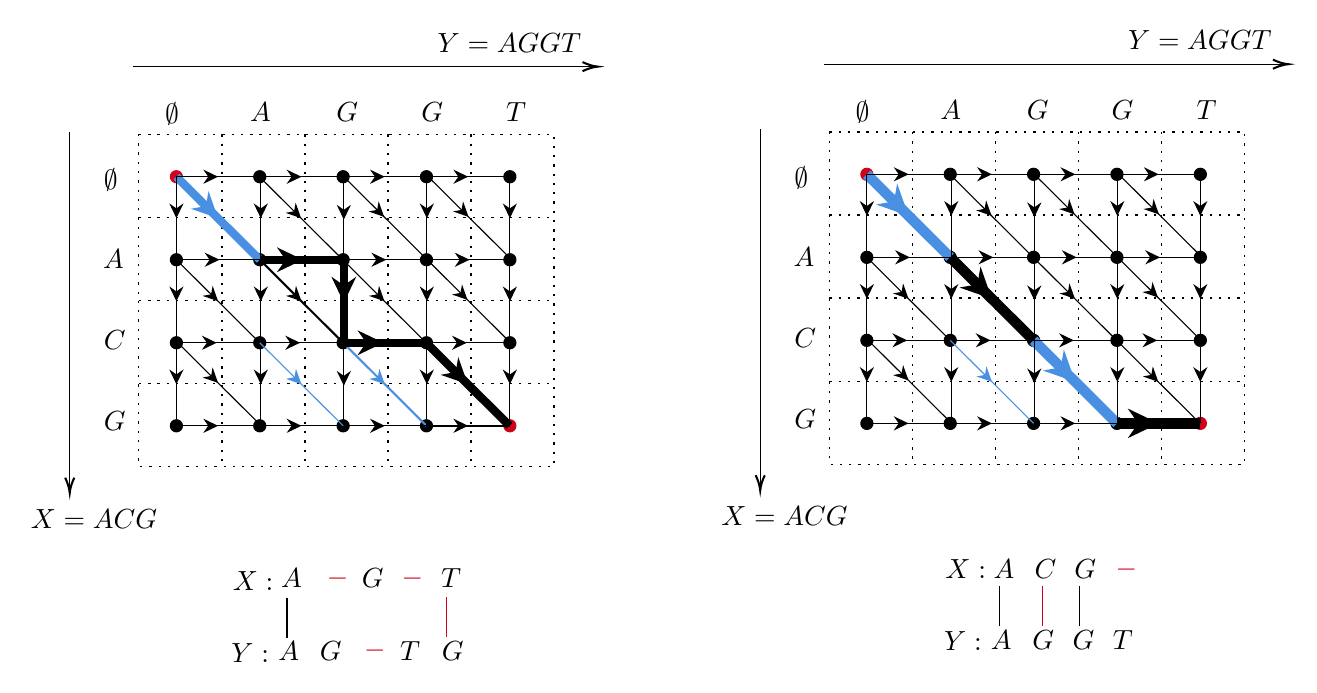
\begin{tikzpicture}[x=0.5pt,y=0.5pt,yscale=-1,xscale=1]
%uncomment if require: \path (0,494); %set diagram left start at 0, and has height of 494

%Shape: Grid [id:dp9095284515127875] 
\draw  [draw opacity=0][dash pattern={on 0.84pt off 2.51pt}] (622,94) -- (922,94) -- (922,334) -- (622,334) -- cycle ; \draw  [dash pattern={on 0.84pt off 2.51pt}] (682,94) -- (682,334)(742,94) -- (742,334)(802,94) -- (802,334)(862,94) -- (862,334) ; \draw  [dash pattern={on 0.84pt off 2.51pt}] (622,154) -- (922,154)(622,214) -- (922,214)(622,274) -- (922,274) ; \draw  [dash pattern={on 0.84pt off 2.51pt}] (622,94) -- (922,94) -- (922,334) -- (622,334) -- cycle ;
%Straight Lines [id:da5347307434268296] 
\draw    (572,92) -- (572,351) ;
\draw [shift={(572,353)}, rotate = 270] [color={rgb, 255:red, 0; green, 0; blue, 0 }  ][line width=0.75]    (10.93,-3.29) .. controls (6.95,-1.4) and (3.31,-0.3) .. (0,0) .. controls (3.31,0.3) and (6.95,1.4) .. (10.93,3.29)   ;
%Straight Lines [id:da4989887299865372] 
\draw    (618,45) -- (951.5,45) ;
\draw [shift={(953.5,45)}, rotate = 180] [color={rgb, 255:red, 0; green, 0; blue, 0 }  ][line width=0.75]    (10.93,-3.29) .. controls (6.95,-1.4) and (3.31,-0.3) .. (0,0) .. controls (3.31,0.3) and (6.95,1.4) .. (10.93,3.29)   ;
%Flowchart: Connector [id:dp7892032191057772] 
\draw  [color={rgb, 255:red, 208; green, 2; blue, 27 }  ,draw opacity=1 ][fill={rgb, 255:red, 208; green, 2; blue, 27 }  ,fill opacity=1 ] (645,123) .. controls (645.87,120.74) and (648.4,119.62) .. (650.66,120.49) .. controls (652.91,121.36) and (654.04,123.89) .. (653.17,126.15) .. controls (652.3,128.4) and (649.77,129.53) .. (647.51,128.66) .. controls (645.26,127.79) and (644.13,125.26) .. (645,123) -- cycle ;
%Flowchart: Connector [id:dp49117478027570705] 
\draw  [fill={rgb, 255:red, 0; green, 0; blue, 0 }  ,fill opacity=1 ] (705.25,123) .. controls (706.11,120.74) and (708.65,119.62) .. (710.9,120.49) .. controls (713.16,121.36) and (714.28,123.89) .. (713.41,126.15) .. controls (712.54,128.4) and (710.01,129.53) .. (707.76,128.66) .. controls (705.5,127.79) and (704.38,125.26) .. (705.25,123) -- cycle ;
%Flowchart: Connector [id:dp26507656226704346] 
\draw  [fill={rgb, 255:red, 0; green, 0; blue, 0 }  ,fill opacity=1 ] (765.49,123) .. controls (766.36,120.74) and (768.89,119.62) .. (771.15,120.49) .. controls (773.4,121.36) and (774.53,123.89) .. (773.66,126.15) .. controls (772.79,128.4) and (770.26,129.53) .. (768,128.66) .. controls (765.75,127.79) and (764.62,125.26) .. (765.49,123) -- cycle ;
%Flowchart: Connector [id:dp5898833817102163] 
\draw  [fill={rgb, 255:red, 0; green, 0; blue, 0 }  ,fill opacity=1 ] (825.74,123) .. controls (826.6,120.74) and (829.14,119.62) .. (831.39,120.49) .. controls (833.65,121.36) and (834.77,123.89) .. (833.9,126.15) .. controls (833.03,128.4) and (830.5,129.53) .. (828.25,128.66) .. controls (825.99,127.79) and (824.87,125.26) .. (825.74,123) -- cycle ;
%Flowchart: Connector [id:dp6978330041031003] 
\draw  [fill={rgb, 255:red, 0; green, 0; blue, 0 }  ,fill opacity=1 ] (886,123) .. controls (886.87,120.74) and (889.4,119.62) .. (891.66,120.49) .. controls (893.91,121.36) and (895.04,123.89) .. (894.17,126.15) .. controls (893.3,128.4) and (890.77,129.53) .. (888.51,128.66) .. controls (886.26,127.79) and (885.13,125.26) .. (886,123) -- cycle ;
%Flowchart: Connector [id:dp8787867823869434] 
\draw  [fill={rgb, 255:red, 0; green, 0; blue, 0 }  ,fill opacity=1 ] (645,183) .. controls (645.87,180.74) and (648.4,179.62) .. (650.66,180.48) .. controls (652.91,181.35) and (654.04,183.89) .. (653.17,186.14) .. controls (652.3,188.4) and (649.77,189.52) .. (647.51,188.65) .. controls (645.26,187.78) and (644.13,185.25) .. (645,183) -- cycle ;
%Flowchart: Connector [id:dp0009714153628327393] 
\draw  [fill={rgb, 255:red, 0; green, 0; blue, 0 }  ,fill opacity=1 ] (705.25,183) .. controls (706.11,180.74) and (708.65,179.62) .. (710.9,180.48) .. controls (713.16,181.35) and (714.28,183.89) .. (713.41,186.14) .. controls (712.54,188.4) and (710.01,189.52) .. (707.76,188.65) .. controls (705.5,187.78) and (704.38,185.25) .. (705.25,183) -- cycle ;
%Flowchart: Connector [id:dp9618763382927992] 
\draw  [fill={rgb, 255:red, 0; green, 0; blue, 0 }  ,fill opacity=1 ] (765.49,183) .. controls (766.36,180.74) and (768.89,179.62) .. (771.15,180.48) .. controls (773.4,181.35) and (774.53,183.89) .. (773.66,186.14) .. controls (772.79,188.4) and (770.26,189.52) .. (768,188.65) .. controls (765.75,187.78) and (764.62,185.25) .. (765.49,183) -- cycle ;
%Flowchart: Connector [id:dp9943373545221997] 
\draw  [fill={rgb, 255:red, 0; green, 0; blue, 0 }  ,fill opacity=1 ] (825.74,183) .. controls (826.6,180.74) and (829.14,179.62) .. (831.39,180.48) .. controls (833.65,181.35) and (834.77,183.89) .. (833.9,186.14) .. controls (833.03,188.4) and (830.5,189.52) .. (828.25,188.65) .. controls (825.99,187.78) and (824.87,185.25) .. (825.74,183) -- cycle ;
%Flowchart: Connector [id:dp482699380394507] 
\draw  [fill={rgb, 255:red, 0; green, 0; blue, 0 }  ,fill opacity=1 ] (886,183) .. controls (886.87,180.74) and (889.4,179.62) .. (891.66,180.48) .. controls (893.91,181.35) and (895.04,183.89) .. (894.17,186.14) .. controls (893.3,188.4) and (890.77,189.52) .. (888.51,188.65) .. controls (886.26,187.78) and (885.13,185.25) .. (886,183) -- cycle ;

%Flowchart: Connector [id:dp7087606993451726] 
\draw  [fill={rgb, 255:red, 0; green, 0; blue, 0 }  ,fill opacity=1 ] (645,242.99) .. controls (645.87,240.73) and (648.4,239.61) .. (650.66,240.48) .. controls (652.91,241.35) and (654.04,243.88) .. (653.17,246.14) .. controls (652.3,248.39) and (649.77,249.52) .. (647.51,248.65) .. controls (645.26,247.78) and (644.13,245.25) .. (645,242.99) -- cycle ;
%Flowchart: Connector [id:dp38414449021330055] 
\draw  [fill={rgb, 255:red, 0; green, 0; blue, 0 }  ,fill opacity=1 ] (705.25,242.99) .. controls (706.11,240.73) and (708.65,239.61) .. (710.9,240.48) .. controls (713.16,241.35) and (714.28,243.88) .. (713.41,246.14) .. controls (712.54,248.39) and (710.01,249.52) .. (707.76,248.65) .. controls (705.5,247.78) and (704.38,245.25) .. (705.25,242.99) -- cycle ;
%Flowchart: Connector [id:dp2499479633678482] 
\draw  [fill={rgb, 255:red, 0; green, 0; blue, 0 }  ,fill opacity=1 ] (765.49,242.99) .. controls (766.36,240.73) and (768.89,239.61) .. (771.15,240.48) .. controls (773.4,241.35) and (774.53,243.88) .. (773.66,246.14) .. controls (772.79,248.39) and (770.26,249.52) .. (768,248.65) .. controls (765.75,247.78) and (764.62,245.25) .. (765.49,242.99) -- cycle ;
%Flowchart: Connector [id:dp3150236979186747] 
\draw  [fill={rgb, 255:red, 0; green, 0; blue, 0 }  ,fill opacity=1 ] (825.74,242.99) .. controls (826.6,240.73) and (829.14,239.61) .. (831.39,240.48) .. controls (833.65,241.35) and (834.77,243.88) .. (833.9,246.14) .. controls (833.03,248.39) and (830.5,249.52) .. (828.25,248.65) .. controls (825.99,247.78) and (824.87,245.25) .. (825.74,242.99) -- cycle ;
%Flowchart: Connector [id:dp5548250717430041] 
\draw  [fill={rgb, 255:red, 0; green, 0; blue, 0 }  ,fill opacity=1 ] (886,242.99) .. controls (886.87,240.73) and (889.4,239.61) .. (891.66,240.48) .. controls (893.91,241.35) and (895.04,243.88) .. (894.17,246.14) .. controls (893.3,248.39) and (890.77,249.52) .. (888.51,248.65) .. controls (886.26,247.78) and (885.13,245.25) .. (886,242.99) -- cycle ;

%Flowchart: Connector [id:dp6724053862379229] 
\draw  [fill={rgb, 255:red, 0; green, 0; blue, 0 }  ,fill opacity=1 ] (645,303) .. controls (645.87,300.74) and (648.4,299.62) .. (650.66,300.49) .. controls (652.91,301.36) and (654.04,303.89) .. (653.17,306.15) .. controls (652.3,308.4) and (649.77,309.53) .. (647.51,308.66) .. controls (645.26,307.79) and (644.13,305.26) .. (645,303) -- cycle ;
%Flowchart: Connector [id:dp809285050914335] 
\draw  [fill={rgb, 255:red, 0; green, 0; blue, 0 }  ,fill opacity=1 ] (705.25,303) .. controls (706.11,300.74) and (708.65,299.62) .. (710.9,300.49) .. controls (713.16,301.36) and (714.28,303.89) .. (713.41,306.15) .. controls (712.54,308.4) and (710.01,309.53) .. (707.76,308.66) .. controls (705.5,307.79) and (704.38,305.26) .. (705.25,303) -- cycle ;
%Flowchart: Connector [id:dp1943046479465117] 
\draw  [fill={rgb, 255:red, 0; green, 0; blue, 0 }  ,fill opacity=1 ] (765.49,303) .. controls (766.36,300.74) and (768.89,299.62) .. (771.15,300.49) .. controls (773.4,301.36) and (774.53,303.89) .. (773.66,306.15) .. controls (772.79,308.4) and (770.26,309.53) .. (768,308.66) .. controls (765.75,307.79) and (764.62,305.26) .. (765.49,303) -- cycle ;
%Flowchart: Connector [id:dp17706594266241393] 
\draw  [fill={rgb, 255:red, 0; green, 0; blue, 0 }  ,fill opacity=1 ] (825.74,303) .. controls (826.6,300.74) and (829.14,299.62) .. (831.39,300.49) .. controls (833.65,301.36) and (834.77,303.89) .. (833.9,306.15) .. controls (833.03,308.4) and (830.5,309.53) .. (828.25,308.66) .. controls (825.99,307.79) and (824.87,305.26) .. (825.74,303) -- cycle ;
%Flowchart: Connector [id:dp06123722582552604] 
\draw  [color={rgb, 255:red, 208; green, 2; blue, 27 }  ,draw opacity=1 ][fill={rgb, 255:red, 208; green, 2; blue, 27 }  ,fill opacity=1 ] (886,303) .. controls (886.87,300.74) and (889.4,299.62) .. (891.66,300.49) .. controls (893.91,301.36) and (895.04,303.89) .. (894.17,306.15) .. controls (893.3,308.4) and (890.77,309.53) .. (888.51,308.66) .. controls (886.26,307.79) and (885.13,305.26) .. (886,303) -- cycle ;
%Straight Lines [id:da3592419747103084] 
\draw [color={rgb, 255:red, 74; green, 144; blue, 226 }  ,draw opacity=1 ][line width=3.75]    (649.08,124.57) -- (709.33,184.57) ;
\draw [shift={(679.21,154.57)}, rotate = 224.88] [fill={rgb, 255:red, 74; green, 144; blue, 226 }  ,fill opacity=1 ][line width=0.08]  [draw opacity=0] (22.33,-10.72) -- (0,0) -- (22.33,10.73) -- (14.83,0) -- cycle    ;
%Straight Lines [id:da11016791165620432] 
\draw [line width=3.75]    (709.33,184.57) -- (769.57,244.56) ;
\draw [shift={(739.45,214.57)}, rotate = 224.88] [fill={rgb, 255:red, 0; green, 0; blue, 0 }  ][line width=0.08]  [draw opacity=0] (22.33,-10.72) -- (0,0) -- (22.33,10.73) -- (14.83,0) -- cycle    ;
%Straight Lines [id:da861324040374141] 
\draw [color={rgb, 255:red, 74; green, 144; blue, 226 }  ,draw opacity=1 ][line width=3.75]    (769.57,244.56) -- (829.82,304.56) ;
\draw [shift={(799.7,274.56)}, rotate = 224.88] [fill={rgb, 255:red, 74; green, 144; blue, 226 }  ,fill opacity=1 ][line width=0.08]  [draw opacity=0] (22.33,-10.72) -- (0,0) -- (22.33,10.73) -- (14.83,0) -- cycle    ;
%Straight Lines [id:da623241069163482] 
\draw    (649.08,124.57) -- (709.33,124.57) ;
\draw [shift={(679.21,124.57)}, rotate = 180] [fill={rgb, 255:red, 0; green, 0; blue, 0 }  ][line width=0.08]  [draw opacity=0] (10.72,-5.15) -- (0,0) -- (10.72,5.15) -- (7.12,0) -- cycle    ;
%Straight Lines [id:da6849986890026631] 
\draw    (709.33,124.57) -- (769.57,124.57) ;
\draw [shift={(739.45,124.57)}, rotate = 180] [fill={rgb, 255:red, 0; green, 0; blue, 0 }  ][line width=0.08]  [draw opacity=0] (10.72,-5.15) -- (0,0) -- (10.72,5.15) -- (7.12,0) -- cycle    ;
%Straight Lines [id:da041846349377336334] 
\draw    (769.57,124.57) -- (829.82,124.57) ;
\draw [shift={(799.7,124.57)}, rotate = 180] [fill={rgb, 255:red, 0; green, 0; blue, 0 }  ][line width=0.08]  [draw opacity=0] (10.72,-5.15) -- (0,0) -- (10.72,5.15) -- (7.12,0) -- cycle    ;
%Straight Lines [id:da39569790466634525] 
\draw    (829.82,124.57) -- (890.06,124.57) ;
\draw [shift={(859.94,124.57)}, rotate = 180] [fill={rgb, 255:red, 0; green, 0; blue, 0 }  ][line width=0.08]  [draw opacity=0] (10.72,-5.15) -- (0,0) -- (10.72,5.15) -- (7.12,0) -- cycle    ;
%Straight Lines [id:da03525501140121612] 
\draw    (650.08,184.57) -- (710.33,184.57) ;
\draw [shift={(680.21,184.57)}, rotate = 180] [fill={rgb, 255:red, 0; green, 0; blue, 0 }  ][line width=0.08]  [draw opacity=0] (10.72,-5.15) -- (0,0) -- (10.72,5.15) -- (7.12,0) -- cycle    ;
%Straight Lines [id:da5053376972804251] 
\draw    (710.33,184.57) -- (770.57,184.57) ;
\draw [shift={(740.45,184.57)}, rotate = 180] [fill={rgb, 255:red, 0; green, 0; blue, 0 }  ][line width=0.08]  [draw opacity=0] (10.72,-5.15) -- (0,0) -- (10.72,5.15) -- (7.12,0) -- cycle    ;
%Straight Lines [id:da9403450630282508] 
\draw    (770.57,184.57) -- (830.82,184.57) ;
\draw [shift={(800.7,184.57)}, rotate = 180] [fill={rgb, 255:red, 0; green, 0; blue, 0 }  ][line width=0.08]  [draw opacity=0] (10.72,-5.15) -- (0,0) -- (10.72,5.15) -- (7.12,0) -- cycle    ;
%Straight Lines [id:da8252476547397996] 
\draw    (830.82,184.57) -- (891.06,184.57) ;
\draw [shift={(860.94,184.57)}, rotate = 180] [fill={rgb, 255:red, 0; green, 0; blue, 0 }  ][line width=0.08]  [draw opacity=0] (10.72,-5.15) -- (0,0) -- (10.72,5.15) -- (7.12,0) -- cycle    ;
%Straight Lines [id:da20328228934926562] 
\draw    (648.08,244.57) -- (708.33,244.57) ;
\draw [shift={(678.21,244.57)}, rotate = 180] [fill={rgb, 255:red, 0; green, 0; blue, 0 }  ][line width=0.08]  [draw opacity=0] (10.72,-5.15) -- (0,0) -- (10.72,5.15) -- (7.12,0) -- cycle    ;
%Straight Lines [id:da18936177213663397] 
\draw    (708.33,244.57) -- (768.57,244.57) ;
\draw [shift={(738.45,244.57)}, rotate = 180] [fill={rgb, 255:red, 0; green, 0; blue, 0 }  ][line width=0.08]  [draw opacity=0] (10.72,-5.15) -- (0,0) -- (10.72,5.15) -- (7.12,0) -- cycle    ;
%Straight Lines [id:da5472813253116537] 
\draw    (768.57,244.57) -- (828.82,244.57) ;
\draw [shift={(798.7,244.57)}, rotate = 180] [fill={rgb, 255:red, 0; green, 0; blue, 0 }  ][line width=0.08]  [draw opacity=0] (10.72,-5.15) -- (0,0) -- (10.72,5.15) -- (7.12,0) -- cycle    ;
%Straight Lines [id:da18891264531279117] 
\draw    (828.82,244.57) -- (889.06,244.57) ;
\draw [shift={(858.94,244.57)}, rotate = 180] [fill={rgb, 255:red, 0; green, 0; blue, 0 }  ][line width=0.08]  [draw opacity=0] (10.72,-5.15) -- (0,0) -- (10.72,5.15) -- (7.12,0) -- cycle    ;
%Straight Lines [id:da39657569614796095] 
\draw    (649.08,304.57) -- (709.33,304.57) ;
\draw [shift={(679.21,304.57)}, rotate = 180] [fill={rgb, 255:red, 0; green, 0; blue, 0 }  ][line width=0.08]  [draw opacity=0] (10.72,-5.15) -- (0,0) -- (10.72,5.15) -- (7.12,0) -- cycle    ;
%Straight Lines [id:da3308363661164806] 
\draw    (709.33,304.57) -- (769.57,304.57) ;
\draw [shift={(739.45,304.57)}, rotate = 180] [fill={rgb, 255:red, 0; green, 0; blue, 0 }  ][line width=0.08]  [draw opacity=0] (10.72,-5.15) -- (0,0) -- (10.72,5.15) -- (7.12,0) -- cycle    ;
%Straight Lines [id:da899869033517725] 
\draw    (769.57,304.57) -- (829.82,304.57) ;
\draw [shift={(799.7,304.57)}, rotate = 180] [fill={rgb, 255:red, 0; green, 0; blue, 0 }  ][line width=0.08]  [draw opacity=0] (10.72,-5.15) -- (0,0) -- (10.72,5.15) -- (7.12,0) -- cycle    ;
%Straight Lines [id:da9491468552348531] 
\draw [line width=3.75]    (829.82,304.57) -- (890.06,304.57) ;
\draw [shift={(859.94,304.57)}, rotate = 180] [fill={rgb, 255:red, 0; green, 0; blue, 0 }  ][line width=0.08]  [draw opacity=0] (22.33,-10.72) -- (0,0) -- (22.33,10.73) -- (14.83,0) -- cycle    ;
%Straight Lines [id:da5447577825869346] 
\draw    (649.08,124.57) -- (649.08,184.57) ;
\draw [shift={(649.08,154.57)}, rotate = 270] [fill={rgb, 255:red, 0; green, 0; blue, 0 }  ][line width=0.08]  [draw opacity=0] (10.72,-5.15) -- (0,0) -- (10.72,5.15) -- (7.12,0) -- cycle    ;
%Straight Lines [id:da4468689576120938] 
\draw    (649.08,184.57) -- (649.08,244.56) ;
\draw [shift={(649.08,214.57)}, rotate = 270] [fill={rgb, 255:red, 0; green, 0; blue, 0 }  ][line width=0.08]  [draw opacity=0] (10.72,-5.15) -- (0,0) -- (10.72,5.15) -- (7.12,0) -- cycle    ;
%Straight Lines [id:da7974322408910806] 
\draw    (649.08,244.58) -- (649.08,304.57) ;
\draw [shift={(649.08,274.58)}, rotate = 270] [fill={rgb, 255:red, 0; green, 0; blue, 0 }  ][line width=0.08]  [draw opacity=0] (10.72,-5.15) -- (0,0) -- (10.72,5.15) -- (7.12,0) -- cycle    ;
%Straight Lines [id:da3348650527968928] 
\draw    (710.08,124.57) -- (710.08,184.57) ;
\draw [shift={(710.08,154.57)}, rotate = 270] [fill={rgb, 255:red, 0; green, 0; blue, 0 }  ][line width=0.08]  [draw opacity=0] (10.72,-5.15) -- (0,0) -- (10.72,5.15) -- (7.12,0) -- cycle    ;
%Straight Lines [id:da506734157691636] 
\draw    (710.08,184.57) -- (710.08,244.56) ;
\draw [shift={(710.08,214.57)}, rotate = 270] [fill={rgb, 255:red, 0; green, 0; blue, 0 }  ][line width=0.08]  [draw opacity=0] (10.72,-5.15) -- (0,0) -- (10.72,5.15) -- (7.12,0) -- cycle    ;
%Straight Lines [id:da5840193538092129] 
\draw    (710.08,244.58) -- (710.08,304.57) ;
\draw [shift={(710.08,274.58)}, rotate = 270] [fill={rgb, 255:red, 0; green, 0; blue, 0 }  ][line width=0.08]  [draw opacity=0] (10.72,-5.15) -- (0,0) -- (10.72,5.15) -- (7.12,0) -- cycle    ;
%Straight Lines [id:da23886443798971468] 
\draw    (770.08,125.57) -- (770.08,185.57) ;
\draw [shift={(770.08,155.57)}, rotate = 270] [fill={rgb, 255:red, 0; green, 0; blue, 0 }  ][line width=0.08]  [draw opacity=0] (10.72,-5.15) -- (0,0) -- (10.72,5.15) -- (7.12,0) -- cycle    ;
%Straight Lines [id:da7044289327291252] 
\draw    (770.08,185.57) -- (770.08,245.56) ;
\draw [shift={(770.08,215.57)}, rotate = 270] [fill={rgb, 255:red, 0; green, 0; blue, 0 }  ][line width=0.08]  [draw opacity=0] (10.72,-5.15) -- (0,0) -- (10.72,5.15) -- (7.12,0) -- cycle    ;
%Straight Lines [id:da3233842191612859] 
\draw    (770.08,245.58) -- (770.08,305.57) ;
\draw [shift={(770.08,275.58)}, rotate = 270] [fill={rgb, 255:red, 0; green, 0; blue, 0 }  ][line width=0.08]  [draw opacity=0] (10.72,-5.15) -- (0,0) -- (10.72,5.15) -- (7.12,0) -- cycle    ;
%Straight Lines [id:da2719581099277214] 
\draw    (830.08,124.57) -- (830.08,184.57) ;
\draw [shift={(830.08,154.57)}, rotate = 270] [fill={rgb, 255:red, 0; green, 0; blue, 0 }  ][line width=0.08]  [draw opacity=0] (10.72,-5.15) -- (0,0) -- (10.72,5.15) -- (7.12,0) -- cycle    ;
%Straight Lines [id:da7955951831524506] 
\draw    (830.08,184.57) -- (830.08,244.56) ;
\draw [shift={(830.08,214.57)}, rotate = 270] [fill={rgb, 255:red, 0; green, 0; blue, 0 }  ][line width=0.08]  [draw opacity=0] (10.72,-5.15) -- (0,0) -- (10.72,5.15) -- (7.12,0) -- cycle    ;
%Straight Lines [id:da5413316975942024] 
\draw    (830.08,244.58) -- (830.08,304.57) ;
\draw [shift={(830.08,274.58)}, rotate = 270] [fill={rgb, 255:red, 0; green, 0; blue, 0 }  ][line width=0.08]  [draw opacity=0] (10.72,-5.15) -- (0,0) -- (10.72,5.15) -- (7.12,0) -- cycle    ;
%Straight Lines [id:da528683157094314] 
\draw    (890.08,124.57) -- (890.08,184.57) ;
\draw [shift={(890.08,154.57)}, rotate = 270] [fill={rgb, 255:red, 0; green, 0; blue, 0 }  ][line width=0.08]  [draw opacity=0] (10.72,-5.15) -- (0,0) -- (10.72,5.15) -- (7.12,0) -- cycle    ;
%Straight Lines [id:da7884969890323227] 
\draw    (890.08,184.57) -- (890.08,244.56) ;
\draw [shift={(890.08,214.57)}, rotate = 270] [fill={rgb, 255:red, 0; green, 0; blue, 0 }  ][line width=0.08]  [draw opacity=0] (10.72,-5.15) -- (0,0) -- (10.72,5.15) -- (7.12,0) -- cycle    ;
%Straight Lines [id:da026306147500106514] 
\draw    (890.08,244.58) -- (890.08,304.57) ;
\draw [shift={(890.08,274.58)}, rotate = 270] [fill={rgb, 255:red, 0; green, 0; blue, 0 }  ][line width=0.08]  [draw opacity=0] (10.72,-5.15) -- (0,0) -- (10.72,5.15) -- (7.12,0) -- cycle    ;
%Straight Lines [id:da5304148083854859] 
\draw    (709.08,124.57) -- (769.33,184.57) ;
\draw [shift={(739.21,154.57)}, rotate = 224.88] [fill={rgb, 255:red, 0; green, 0; blue, 0 }  ][line width=0.08]  [draw opacity=0] (10.72,-5.15) -- (0,0) -- (10.72,5.15) -- (7.12,0) -- cycle    ;
%Straight Lines [id:da10387619856914898] 
\draw    (769.33,184.57) -- (829.57,244.56) ;
\draw [shift={(799.45,214.57)}, rotate = 224.88] [fill={rgb, 255:red, 0; green, 0; blue, 0 }  ][line width=0.08]  [draw opacity=0] (10.72,-5.15) -- (0,0) -- (10.72,5.15) -- (7.12,0) -- cycle    ;
%Straight Lines [id:da6684466112396508] 
\draw    (829.57,244.56) -- (889.82,304.56) ;
\draw [shift={(859.7,274.56)}, rotate = 224.88] [fill={rgb, 255:red, 0; green, 0; blue, 0 }  ][line width=0.08]  [draw opacity=0] (10.72,-5.15) -- (0,0) -- (10.72,5.15) -- (7.12,0) -- cycle    ;
%Straight Lines [id:da3445451700183738] 
\draw    (769.08,123.57) -- (829.33,183.57) ;
\draw [shift={(799.21,153.57)}, rotate = 224.88] [fill={rgb, 255:red, 0; green, 0; blue, 0 }  ][line width=0.08]  [draw opacity=0] (10.72,-5.15) -- (0,0) -- (10.72,5.15) -- (7.12,0) -- cycle    ;
%Straight Lines [id:da9388081629332891] 
\draw    (829.33,183.57) -- (889.57,243.56) ;
\draw [shift={(859.45,213.57)}, rotate = 224.88] [fill={rgb, 255:red, 0; green, 0; blue, 0 }  ][line width=0.08]  [draw opacity=0] (10.72,-5.15) -- (0,0) -- (10.72,5.15) -- (7.12,0) -- cycle    ;
%Straight Lines [id:da5665052547166216] 
\draw    (830.08,123.57) -- (890.33,183.57) ;
\draw [shift={(860.21,153.57)}, rotate = 224.88] [fill={rgb, 255:red, 0; green, 0; blue, 0 }  ][line width=0.08]  [draw opacity=0] (10.72,-5.15) -- (0,0) -- (10.72,5.15) -- (7.12,0) -- cycle    ;
%Straight Lines [id:da5547716631608589] 
\draw    (649.08,184.57) -- (709.33,244.57) ;
\draw [shift={(679.21,214.57)}, rotate = 224.88] [fill={rgb, 255:red, 0; green, 0; blue, 0 }  ][line width=0.08]  [draw opacity=0] (10.72,-5.15) -- (0,0) -- (10.72,5.15) -- (7.12,0) -- cycle    ;
%Straight Lines [id:da44797690158878345] 
\draw [color={rgb, 255:red, 74; green, 144; blue, 226 }  ,draw opacity=1 ]   (709.33,244.57) -- (769.57,304.56) ;
\draw [shift={(739.45,274.57)}, rotate = 224.88] [fill={rgb, 255:red, 74; green, 144; blue, 226 }  ,fill opacity=1 ][line width=0.08]  [draw opacity=0] (10.72,-5.15) -- (0,0) -- (10.72,5.15) -- (7.12,0) -- cycle    ;
%Straight Lines [id:da4158633112708935] 
\draw    (649.08,243.57) -- (709.33,303.57) ;
\draw [shift={(679.21,273.57)}, rotate = 224.88] [fill={rgb, 255:red, 0; green, 0; blue, 0 }  ][line width=0.08]  [draw opacity=0] (10.72,-5.15) -- (0,0) -- (10.72,5.15) -- (7.12,0) -- cycle    ;
%Straight Lines [id:da17724026714082763] 
\draw    (745,422) -- (745,451) ;
%Straight Lines [id:da7508046419845208] 
\draw [color={rgb, 255:red, 208; green, 2; blue, 27 }  ,draw opacity=1 ]   (776,422) -- (776,451) ;
%Straight Lines [id:da2544301147710125] 
\draw [color={rgb, 255:red, 0; green, 0; blue, 0 }  ,draw opacity=1 ]   (803,422) -- (803,451) ;
%Straight Lines [id:da8541738900783582] 
\draw    (230,430.75) -- (230,459.75) ;
%Straight Lines [id:da050432862458620886] 
\draw [color={rgb, 255:red, 208; green, 2; blue, 27 }  ,draw opacity=1 ]   (345,429.75) -- (345,458.75) ;
%Shape: Grid [id:dp27190276733655694] 
\draw  [draw opacity=0][dash pattern={on 0.84pt off 2.51pt}] (123,95.75) -- (423,95.75) -- (423,335.75) -- (123,335.75) -- cycle ; \draw  [dash pattern={on 0.84pt off 2.51pt}] (183,95.75) -- (183,335.75)(243,95.75) -- (243,335.75)(303,95.75) -- (303,335.75)(363,95.75) -- (363,335.75) ; \draw  [dash pattern={on 0.84pt off 2.51pt}] (123,155.75) -- (423,155.75)(123,215.75) -- (423,215.75)(123,275.75) -- (423,275.75) ; \draw  [dash pattern={on 0.84pt off 2.51pt}] (123,95.75) -- (423,95.75) -- (423,335.75) -- (123,335.75) -- cycle ;
%Straight Lines [id:da7174522079484525] 
\draw    (73,93.75) -- (73,352.75) ;
\draw [shift={(73,354.75)}, rotate = 270] [color={rgb, 255:red, 0; green, 0; blue, 0 }  ][line width=0.75]    (10.93,-3.29) .. controls (6.95,-1.4) and (3.31,-0.3) .. (0,0) .. controls (3.31,0.3) and (6.95,1.4) .. (10.93,3.29)   ;
%Straight Lines [id:da7367836278004803] 
\draw    (119,46.75) -- (452.5,46.75) ;
\draw [shift={(454.5,46.75)}, rotate = 180] [color={rgb, 255:red, 0; green, 0; blue, 0 }  ][line width=0.75]    (10.93,-3.29) .. controls (6.95,-1.4) and (3.31,-0.3) .. (0,0) .. controls (3.31,0.3) and (6.95,1.4) .. (10.93,3.29)   ;
%Flowchart: Connector [id:dp8743229494742727] 
\draw  [color={rgb, 255:red, 208; green, 2; blue, 27 }  ,draw opacity=1 ][fill={rgb, 255:red, 208; green, 2; blue, 27 }  ,fill opacity=1 ] (146,124.75) .. controls (146.87,122.49) and (149.4,121.37) .. (151.66,122.24) .. controls (153.91,123.11) and (155.04,125.64) .. (154.17,127.9) .. controls (153.3,130.15) and (150.77,131.28) .. (148.51,130.41) .. controls (146.26,129.54) and (145.13,127.01) .. (146,124.75) -- cycle ;
%Flowchart: Connector [id:dp8049838465641742] 
\draw  [fill={rgb, 255:red, 0; green, 0; blue, 0 }  ,fill opacity=1 ] (206.25,124.75) .. controls (207.11,122.49) and (209.65,121.37) .. (211.9,122.24) .. controls (214.16,123.11) and (215.28,125.64) .. (214.41,127.9) .. controls (213.54,130.15) and (211.01,131.28) .. (208.76,130.41) .. controls (206.5,129.54) and (205.38,127.01) .. (206.25,124.75) -- cycle ;
%Flowchart: Connector [id:dp329643068959084] 
\draw  [fill={rgb, 255:red, 0; green, 0; blue, 0 }  ,fill opacity=1 ] (266.49,124.75) .. controls (267.36,122.49) and (269.89,121.37) .. (272.15,122.24) .. controls (274.4,123.11) and (275.53,125.64) .. (274.66,127.9) .. controls (273.79,130.15) and (271.26,131.28) .. (269,130.41) .. controls (266.75,129.54) and (265.62,127.01) .. (266.49,124.75) -- cycle ;
%Flowchart: Connector [id:dp5873162391128393] 
\draw  [fill={rgb, 255:red, 0; green, 0; blue, 0 }  ,fill opacity=1 ] (326.74,124.75) .. controls (327.6,122.49) and (330.14,121.37) .. (332.39,122.24) .. controls (334.65,123.11) and (335.77,125.64) .. (334.9,127.9) .. controls (334.03,130.15) and (331.5,131.28) .. (329.25,130.41) .. controls (326.99,129.54) and (325.87,127.01) .. (326.74,124.75) -- cycle ;
%Flowchart: Connector [id:dp7420220767016437] 
\draw  [fill={rgb, 255:red, 0; green, 0; blue, 0 }  ,fill opacity=1 ] (387,124.75) .. controls (387.87,122.49) and (390.4,121.37) .. (392.66,122.24) .. controls (394.91,123.11) and (396.04,125.64) .. (395.17,127.9) .. controls (394.3,130.15) and (391.77,131.28) .. (389.51,130.41) .. controls (387.26,129.54) and (386.13,127.01) .. (387,124.75) -- cycle ;
%Flowchart: Connector [id:dp934195248321976] 
\draw  [fill={rgb, 255:red, 0; green, 0; blue, 0 }  ,fill opacity=1 ] (146,184.75) .. controls (146.87,182.49) and (149.4,181.37) .. (151.66,182.23) .. controls (153.91,183.1) and (155.04,185.64) .. (154.17,187.89) .. controls (153.3,190.15) and (150.77,191.27) .. (148.51,190.4) .. controls (146.26,189.53) and (145.13,187) .. (146,184.75) -- cycle ;
%Flowchart: Connector [id:dp5915793374687792] 
\draw  [fill={rgb, 255:red, 0; green, 0; blue, 0 }  ,fill opacity=1 ] (206.25,184.75) .. controls (207.11,182.49) and (209.65,181.37) .. (211.9,182.23) .. controls (214.16,183.1) and (215.28,185.64) .. (214.41,187.89) .. controls (213.54,190.15) and (211.01,191.27) .. (208.76,190.4) .. controls (206.5,189.53) and (205.38,187) .. (206.25,184.75) -- cycle ;
%Flowchart: Connector [id:dp9212660757973473] 
\draw  [fill={rgb, 255:red, 0; green, 0; blue, 0 }  ,fill opacity=1 ] (266.49,184.75) .. controls (267.36,182.49) and (269.89,181.37) .. (272.15,182.23) .. controls (274.4,183.1) and (275.53,185.64) .. (274.66,187.89) .. controls (273.79,190.15) and (271.26,191.27) .. (269,190.4) .. controls (266.75,189.53) and (265.62,187) .. (266.49,184.75) -- cycle ;
%Flowchart: Connector [id:dp8085932168532495] 
\draw  [fill={rgb, 255:red, 0; green, 0; blue, 0 }  ,fill opacity=1 ] (326.74,184.75) .. controls (327.6,182.49) and (330.14,181.37) .. (332.39,182.23) .. controls (334.65,183.1) and (335.77,185.64) .. (334.9,187.89) .. controls (334.03,190.15) and (331.5,191.27) .. (329.25,190.4) .. controls (326.99,189.53) and (325.87,187) .. (326.74,184.75) -- cycle ;
%Flowchart: Connector [id:dp859886140020651] 
\draw  [fill={rgb, 255:red, 0; green, 0; blue, 0 }  ,fill opacity=1 ] (387,184.75) .. controls (387.87,182.49) and (390.4,181.37) .. (392.66,182.23) .. controls (394.91,183.1) and (396.04,185.64) .. (395.17,187.89) .. controls (394.3,190.15) and (391.77,191.27) .. (389.51,190.4) .. controls (387.26,189.53) and (386.13,187) .. (387,184.75) -- cycle ;

%Flowchart: Connector [id:dp7915454663594278] 
\draw  [fill={rgb, 255:red, 0; green, 0; blue, 0 }  ,fill opacity=1 ] (146,244.74) .. controls (146.87,242.48) and (149.4,241.36) .. (151.66,242.23) .. controls (153.91,243.1) and (155.04,245.63) .. (154.17,247.89) .. controls (153.3,250.14) and (150.77,251.27) .. (148.51,250.4) .. controls (146.26,249.53) and (145.13,247) .. (146,244.74) -- cycle ;
%Flowchart: Connector [id:dp17480431454341216] 
\draw  [fill={rgb, 255:red, 0; green, 0; blue, 0 }  ,fill opacity=1 ] (206.25,244.74) .. controls (207.11,242.48) and (209.65,241.36) .. (211.9,242.23) .. controls (214.16,243.1) and (215.28,245.63) .. (214.41,247.89) .. controls (213.54,250.14) and (211.01,251.27) .. (208.76,250.4) .. controls (206.5,249.53) and (205.38,247) .. (206.25,244.74) -- cycle ;
%Flowchart: Connector [id:dp2536010529258059] 
\draw  [fill={rgb, 255:red, 0; green, 0; blue, 0 }  ,fill opacity=1 ] (266.49,244.74) .. controls (267.36,242.48) and (269.89,241.36) .. (272.15,242.23) .. controls (274.4,243.1) and (275.53,245.63) .. (274.66,247.89) .. controls (273.79,250.14) and (271.26,251.27) .. (269,250.4) .. controls (266.75,249.53) and (265.62,247) .. (266.49,244.74) -- cycle ;
%Flowchart: Connector [id:dp30104810992620934] 
\draw  [fill={rgb, 255:red, 0; green, 0; blue, 0 }  ,fill opacity=1 ] (326.74,244.74) .. controls (327.6,242.48) and (330.14,241.36) .. (332.39,242.23) .. controls (334.65,243.1) and (335.77,245.63) .. (334.9,247.89) .. controls (334.03,250.14) and (331.5,251.27) .. (329.25,250.4) .. controls (326.99,249.53) and (325.87,247) .. (326.74,244.74) -- cycle ;
%Flowchart: Connector [id:dp22547368817934332] 
\draw  [fill={rgb, 255:red, 0; green, 0; blue, 0 }  ,fill opacity=1 ] (387,244.74) .. controls (387.87,242.48) and (390.4,241.36) .. (392.66,242.23) .. controls (394.91,243.1) and (396.04,245.63) .. (395.17,247.89) .. controls (394.3,250.14) and (391.77,251.27) .. (389.51,250.4) .. controls (387.26,249.53) and (386.13,247) .. (387,244.74) -- cycle ;

%Flowchart: Connector [id:dp7621441808209223] 
\draw  [fill={rgb, 255:red, 0; green, 0; blue, 0 }  ,fill opacity=1 ] (146,304.75) .. controls (146.87,302.49) and (149.4,301.37) .. (151.66,302.24) .. controls (153.91,303.11) and (155.04,305.64) .. (154.17,307.9) .. controls (153.3,310.15) and (150.77,311.28) .. (148.51,310.41) .. controls (146.26,309.54) and (145.13,307.01) .. (146,304.75) -- cycle ;
%Flowchart: Connector [id:dp17937394389606287] 
\draw  [fill={rgb, 255:red, 0; green, 0; blue, 0 }  ,fill opacity=1 ] (206.25,304.75) .. controls (207.11,302.49) and (209.65,301.37) .. (211.9,302.24) .. controls (214.16,303.11) and (215.28,305.64) .. (214.41,307.9) .. controls (213.54,310.15) and (211.01,311.28) .. (208.76,310.41) .. controls (206.5,309.54) and (205.38,307.01) .. (206.25,304.75) -- cycle ;
%Flowchart: Connector [id:dp6927820246993454] 
\draw  [fill={rgb, 255:red, 0; green, 0; blue, 0 }  ,fill opacity=1 ] (266.49,304.75) .. controls (267.36,302.49) and (269.89,301.37) .. (272.15,302.24) .. controls (274.4,303.11) and (275.53,305.64) .. (274.66,307.9) .. controls (273.79,310.15) and (271.26,311.28) .. (269,310.41) .. controls (266.75,309.54) and (265.62,307.01) .. (266.49,304.75) -- cycle ;
%Flowchart: Connector [id:dp192571137230252] 
\draw  [fill={rgb, 255:red, 0; green, 0; blue, 0 }  ,fill opacity=1 ] (326.74,304.75) .. controls (327.6,302.49) and (330.14,301.37) .. (332.39,302.24) .. controls (334.65,303.11) and (335.77,305.64) .. (334.9,307.9) .. controls (334.03,310.15) and (331.5,311.28) .. (329.25,310.41) .. controls (326.99,309.54) and (325.87,307.01) .. (326.74,304.75) -- cycle ;
%Flowchart: Connector [id:dp7961764434418737] 
\draw  [color={rgb, 255:red, 208; green, 2; blue, 27 }  ,draw opacity=1 ][fill={rgb, 255:red, 208; green, 2; blue, 27 }  ,fill opacity=1 ] (387,304.75) .. controls (387.87,302.49) and (390.4,301.37) .. (392.66,302.24) .. controls (394.91,303.11) and (396.04,305.64) .. (395.17,307.9) .. controls (394.3,310.15) and (391.77,311.28) .. (389.51,310.41) .. controls (387.26,309.54) and (386.13,307.01) .. (387,304.75) -- cycle ;
%Straight Lines [id:da38641070829975266] 
\draw [color={rgb, 255:red, 74; green, 144; blue, 226 }  ,draw opacity=1 ][line width=3]    (150.08,126.32) -- (210.33,186.32) ;
\draw [shift={(180.21,156.32)}, rotate = 224.88] [fill={rgb, 255:red, 74; green, 144; blue, 226 }  ,fill opacity=1 ][line width=0.08]  [draw opacity=0] (18.75,-9.01) -- (0,0) -- (18.75,9.01) -- (12.45,0) -- cycle    ;
%Straight Lines [id:da3615690240336379] 
\draw [line width=0.75]    (210.33,186.32) -- (270.57,246.31) ;
\draw [shift={(240.45,216.32)}, rotate = 224.88] [fill={rgb, 255:red, 0; green, 0; blue, 0 }  ][line width=0.08]  [draw opacity=0] (10.72,-5.15) -- (0,0) -- (10.72,5.15) -- (7.12,0) -- cycle    ;
%Straight Lines [id:da6165888142013153] 
\draw [color={rgb, 255:red, 74; green, 144; blue, 226 }  ,draw opacity=1 ][line width=0.75]    (270.57,246.31) -- (330.82,306.31) ;
\draw [shift={(300.7,276.31)}, rotate = 224.88] [fill={rgb, 255:red, 74; green, 144; blue, 226 }  ,fill opacity=1 ][line width=0.08]  [draw opacity=0] (10.72,-5.15) -- (0,0) -- (10.72,5.15) -- (7.12,0) -- cycle    ;
%Straight Lines [id:da5468840905017531] 
\draw    (150.08,126.32) -- (210.33,126.32) ;
\draw [shift={(180.21,126.32)}, rotate = 180] [fill={rgb, 255:red, 0; green, 0; blue, 0 }  ][line width=0.08]  [draw opacity=0] (10.72,-5.15) -- (0,0) -- (10.72,5.15) -- (7.12,0) -- cycle    ;
%Straight Lines [id:da8282921785641422] 
\draw    (210.33,126.32) -- (270.57,126.32) ;
\draw [shift={(240.45,126.32)}, rotate = 180] [fill={rgb, 255:red, 0; green, 0; blue, 0 }  ][line width=0.08]  [draw opacity=0] (10.72,-5.15) -- (0,0) -- (10.72,5.15) -- (7.12,0) -- cycle    ;
%Straight Lines [id:da1472752931372323] 
\draw    (270.57,126.32) -- (330.82,126.32) ;
\draw [shift={(300.7,126.32)}, rotate = 180] [fill={rgb, 255:red, 0; green, 0; blue, 0 }  ][line width=0.08]  [draw opacity=0] (10.72,-5.15) -- (0,0) -- (10.72,5.15) -- (7.12,0) -- cycle    ;
%Straight Lines [id:da705641761176685] 
\draw    (330.82,126.32) -- (391.06,126.32) ;
\draw [shift={(360.94,126.32)}, rotate = 180] [fill={rgb, 255:red, 0; green, 0; blue, 0 }  ][line width=0.08]  [draw opacity=0] (10.72,-5.15) -- (0,0) -- (10.72,5.15) -- (7.12,0) -- cycle    ;
%Straight Lines [id:da01614116141903499] 
\draw    (151.08,186.32) -- (211.33,186.32) ;
\draw [shift={(181.21,186.32)}, rotate = 180] [fill={rgb, 255:red, 0; green, 0; blue, 0 }  ][line width=0.08]  [draw opacity=0] (10.72,-5.15) -- (0,0) -- (10.72,5.15) -- (7.12,0) -- cycle    ;
%Straight Lines [id:da18789251927655182] 
\draw [line width=3]    (211.33,186.32) -- (271.57,186.32) ;
\draw [shift={(241.45,186.32)}, rotate = 180] [fill={rgb, 255:red, 0; green, 0; blue, 0 }  ][line width=0.08]  [draw opacity=0] (18.75,-9.01) -- (0,0) -- (18.75,9.01) -- (12.45,0) -- cycle    ;
%Straight Lines [id:da6027501411096107] 
\draw    (271.57,186.32) -- (331.82,186.32) ;
\draw [shift={(301.7,186.32)}, rotate = 180] [fill={rgb, 255:red, 0; green, 0; blue, 0 }  ][line width=0.08]  [draw opacity=0] (10.72,-5.15) -- (0,0) -- (10.72,5.15) -- (7.12,0) -- cycle    ;
%Straight Lines [id:da8504498965643004] 
\draw    (331.82,186.32) -- (392.06,186.32) ;
\draw [shift={(361.94,186.32)}, rotate = 180] [fill={rgb, 255:red, 0; green, 0; blue, 0 }  ][line width=0.08]  [draw opacity=0] (10.72,-5.15) -- (0,0) -- (10.72,5.15) -- (7.12,0) -- cycle    ;
%Straight Lines [id:da5555928745234902] 
\draw    (149.08,246.32) -- (209.33,246.32) ;
\draw [shift={(179.21,246.32)}, rotate = 180] [fill={rgb, 255:red, 0; green, 0; blue, 0 }  ][line width=0.08]  [draw opacity=0] (10.72,-5.15) -- (0,0) -- (10.72,5.15) -- (7.12,0) -- cycle    ;
%Straight Lines [id:da7703345296509445] 
\draw    (209.33,246.32) -- (269.57,246.32) ;
\draw [shift={(239.45,246.32)}, rotate = 180] [fill={rgb, 255:red, 0; green, 0; blue, 0 }  ][line width=0.08]  [draw opacity=0] (10.72,-5.15) -- (0,0) -- (10.72,5.15) -- (7.12,0) -- cycle    ;
%Straight Lines [id:da8121394847539791] 
\draw [line width=3]    (269.57,246.32) -- (329.82,246.32) ;
\draw [shift={(299.7,246.32)}, rotate = 180] [fill={rgb, 255:red, 0; green, 0; blue, 0 }  ][line width=0.08]  [draw opacity=0] (18.75,-9.01) -- (0,0) -- (18.75,9.01) -- (12.45,0) -- cycle    ;
%Straight Lines [id:da026771713494214255] 
\draw    (329.82,246.32) -- (390.06,246.32) ;
\draw [shift={(359.94,246.32)}, rotate = 180] [fill={rgb, 255:red, 0; green, 0; blue, 0 }  ][line width=0.08]  [draw opacity=0] (10.72,-5.15) -- (0,0) -- (10.72,5.15) -- (7.12,0) -- cycle    ;
%Straight Lines [id:da4345037157640508] 
\draw    (150.08,306.32) -- (210.33,306.32) ;
\draw [shift={(180.21,306.32)}, rotate = 180] [fill={rgb, 255:red, 0; green, 0; blue, 0 }  ][line width=0.08]  [draw opacity=0] (10.72,-5.15) -- (0,0) -- (10.72,5.15) -- (7.12,0) -- cycle    ;
%Straight Lines [id:da17363134702975358] 
\draw    (210.33,306.32) -- (270.57,306.32) ;
\draw [shift={(240.45,306.32)}, rotate = 180] [fill={rgb, 255:red, 0; green, 0; blue, 0 }  ][line width=0.08]  [draw opacity=0] (10.72,-5.15) -- (0,0) -- (10.72,5.15) -- (7.12,0) -- cycle    ;
%Straight Lines [id:da4023485747053863] 
\draw    (270.57,306.32) -- (330.82,306.32) ;
\draw [shift={(300.7,306.32)}, rotate = 180] [fill={rgb, 255:red, 0; green, 0; blue, 0 }  ][line width=0.08]  [draw opacity=0] (10.72,-5.15) -- (0,0) -- (10.72,5.15) -- (7.12,0) -- cycle    ;
%Straight Lines [id:da7966143920791751] 
\draw [line width=0.75]    (330.82,306.32) -- (391.06,306.32) ;
\draw [shift={(360.94,306.32)}, rotate = 180] [fill={rgb, 255:red, 0; green, 0; blue, 0 }  ][line width=0.08]  [draw opacity=0] (10.72,-5.15) -- (0,0) -- (10.72,5.15) -- (7.12,0) -- cycle    ;
%Straight Lines [id:da36738171983978807] 
\draw    (150.08,126.32) -- (150.08,186.32) ;
\draw [shift={(150.08,156.32)}, rotate = 270] [fill={rgb, 255:red, 0; green, 0; blue, 0 }  ][line width=0.08]  [draw opacity=0] (10.72,-5.15) -- (0,0) -- (10.72,5.15) -- (7.12,0) -- cycle    ;
%Straight Lines [id:da43784341965789353] 
\draw    (150.08,186.32) -- (150.08,246.31) ;
\draw [shift={(150.08,216.32)}, rotate = 270] [fill={rgb, 255:red, 0; green, 0; blue, 0 }  ][line width=0.08]  [draw opacity=0] (10.72,-5.15) -- (0,0) -- (10.72,5.15) -- (7.12,0) -- cycle    ;
%Straight Lines [id:da21158535824208968] 
\draw    (150.08,246.33) -- (150.08,306.32) ;
\draw [shift={(150.08,276.33)}, rotate = 270] [fill={rgb, 255:red, 0; green, 0; blue, 0 }  ][line width=0.08]  [draw opacity=0] (10.72,-5.15) -- (0,0) -- (10.72,5.15) -- (7.12,0) -- cycle    ;
%Straight Lines [id:da9621218270210167] 
\draw    (211.08,126.32) -- (211.08,186.32) ;
\draw [shift={(211.08,156.32)}, rotate = 270] [fill={rgb, 255:red, 0; green, 0; blue, 0 }  ][line width=0.08]  [draw opacity=0] (10.72,-5.15) -- (0,0) -- (10.72,5.15) -- (7.12,0) -- cycle    ;
%Straight Lines [id:da8767441889455209] 
\draw    (211.08,186.32) -- (211.08,246.31) ;
\draw [shift={(211.08,216.32)}, rotate = 270] [fill={rgb, 255:red, 0; green, 0; blue, 0 }  ][line width=0.08]  [draw opacity=0] (10.72,-5.15) -- (0,0) -- (10.72,5.15) -- (7.12,0) -- cycle    ;
%Straight Lines [id:da8198708978187301] 
\draw    (211.08,246.33) -- (211.08,306.32) ;
\draw [shift={(211.08,276.33)}, rotate = 270] [fill={rgb, 255:red, 0; green, 0; blue, 0 }  ][line width=0.08]  [draw opacity=0] (10.72,-5.15) -- (0,0) -- (10.72,5.15) -- (7.12,0) -- cycle    ;
%Straight Lines [id:da5543023734085751] 
\draw    (271.08,127.32) -- (271.08,187.32) ;
\draw [shift={(271.08,157.32)}, rotate = 270] [fill={rgb, 255:red, 0; green, 0; blue, 0 }  ][line width=0.08]  [draw opacity=0] (10.72,-5.15) -- (0,0) -- (10.72,5.15) -- (7.12,0) -- cycle    ;
%Straight Lines [id:da12739018951386039] 
\draw [line width=3]    (271.08,187.32) -- (271.08,247.31) ;
\draw [shift={(271.08,217.32)}, rotate = 270] [fill={rgb, 255:red, 0; green, 0; blue, 0 }  ][line width=0.08]  [draw opacity=0] (18.75,-9.01) -- (0,0) -- (18.75,9.01) -- (12.45,0) -- cycle    ;
%Straight Lines [id:da25478497800586] 
\draw    (271.08,247.33) -- (271.08,307.32) ;
\draw [shift={(271.08,277.33)}, rotate = 270] [fill={rgb, 255:red, 0; green, 0; blue, 0 }  ][line width=0.08]  [draw opacity=0] (10.72,-5.15) -- (0,0) -- (10.72,5.15) -- (7.12,0) -- cycle    ;
%Straight Lines [id:da8255409504470865] 
\draw    (331.08,126.32) -- (331.08,186.32) ;
\draw [shift={(331.08,156.32)}, rotate = 270] [fill={rgb, 255:red, 0; green, 0; blue, 0 }  ][line width=0.08]  [draw opacity=0] (10.72,-5.15) -- (0,0) -- (10.72,5.15) -- (7.12,0) -- cycle    ;
%Straight Lines [id:da24820069145014834] 
\draw    (331.08,186.32) -- (331.08,246.31) ;
\draw [shift={(331.08,216.32)}, rotate = 270] [fill={rgb, 255:red, 0; green, 0; blue, 0 }  ][line width=0.08]  [draw opacity=0] (10.72,-5.15) -- (0,0) -- (10.72,5.15) -- (7.12,0) -- cycle    ;
%Straight Lines [id:da8406020938464005] 
\draw    (331.08,246.33) -- (331.08,306.32) ;
\draw [shift={(331.08,276.33)}, rotate = 270] [fill={rgb, 255:red, 0; green, 0; blue, 0 }  ][line width=0.08]  [draw opacity=0] (10.72,-5.15) -- (0,0) -- (10.72,5.15) -- (7.12,0) -- cycle    ;
%Straight Lines [id:da12205797133948904] 
\draw    (391.08,126.32) -- (391.08,186.32) ;
\draw [shift={(391.08,156.32)}, rotate = 270] [fill={rgb, 255:red, 0; green, 0; blue, 0 }  ][line width=0.08]  [draw opacity=0] (10.72,-5.15) -- (0,0) -- (10.72,5.15) -- (7.12,0) -- cycle    ;
%Straight Lines [id:da1505370432896579] 
\draw    (391.08,186.32) -- (391.08,246.31) ;
\draw [shift={(391.08,216.32)}, rotate = 270] [fill={rgb, 255:red, 0; green, 0; blue, 0 }  ][line width=0.08]  [draw opacity=0] (10.72,-5.15) -- (0,0) -- (10.72,5.15) -- (7.12,0) -- cycle    ;
%Straight Lines [id:da5221205898449226] 
\draw    (391.08,246.33) -- (391.08,306.32) ;
\draw [shift={(391.08,276.33)}, rotate = 270] [fill={rgb, 255:red, 0; green, 0; blue, 0 }  ][line width=0.08]  [draw opacity=0] (10.72,-5.15) -- (0,0) -- (10.72,5.15) -- (7.12,0) -- cycle    ;
%Straight Lines [id:da6158477075598086] 
\draw    (210.08,126.32) -- (270.33,186.32) ;
\draw [shift={(240.21,156.32)}, rotate = 224.88] [fill={rgb, 255:red, 0; green, 0; blue, 0 }  ][line width=0.08]  [draw opacity=0] (10.72,-5.15) -- (0,0) -- (10.72,5.15) -- (7.12,0) -- cycle    ;
%Straight Lines [id:da01553667248539925] 
\draw    (270.33,186.32) -- (330.57,246.31) ;
\draw [shift={(300.45,216.32)}, rotate = 224.88] [fill={rgb, 255:red, 0; green, 0; blue, 0 }  ][line width=0.08]  [draw opacity=0] (10.72,-5.15) -- (0,0) -- (10.72,5.15) -- (7.12,0) -- cycle    ;
%Straight Lines [id:da4099310076744064] 
\draw [line width=3]    (330.57,246.31) -- (390.82,306.31) ;
\draw [shift={(360.7,276.31)}, rotate = 224.88] [fill={rgb, 255:red, 0; green, 0; blue, 0 }  ][line width=0.08]  [draw opacity=0] (18.75,-9.01) -- (0,0) -- (18.75,9.01) -- (12.45,0) -- cycle    ;
%Straight Lines [id:da9906691147163563] 
\draw    (270.08,125.32) -- (330.33,185.32) ;
\draw [shift={(300.21,155.32)}, rotate = 224.88] [fill={rgb, 255:red, 0; green, 0; blue, 0 }  ][line width=0.08]  [draw opacity=0] (10.72,-5.15) -- (0,0) -- (10.72,5.15) -- (7.12,0) -- cycle    ;
%Straight Lines [id:da7033414065493556] 
\draw    (330.33,185.32) -- (390.57,245.31) ;
\draw [shift={(360.45,215.32)}, rotate = 224.88] [fill={rgb, 255:red, 0; green, 0; blue, 0 }  ][line width=0.08]  [draw opacity=0] (10.72,-5.15) -- (0,0) -- (10.72,5.15) -- (7.12,0) -- cycle    ;
%Straight Lines [id:da8488328983682633] 
\draw    (331.08,125.32) -- (391.33,185.32) ;
\draw [shift={(361.21,155.32)}, rotate = 224.88] [fill={rgb, 255:red, 0; green, 0; blue, 0 }  ][line width=0.08]  [draw opacity=0] (10.72,-5.15) -- (0,0) -- (10.72,5.15) -- (7.12,0) -- cycle    ;
%Straight Lines [id:da4285004266984822] 
\draw    (150.08,186.32) -- (210.33,246.32) ;
\draw [shift={(180.21,216.32)}, rotate = 224.88] [fill={rgb, 255:red, 0; green, 0; blue, 0 }  ][line width=0.08]  [draw opacity=0] (10.72,-5.15) -- (0,0) -- (10.72,5.15) -- (7.12,0) -- cycle    ;
%Straight Lines [id:da7676748719347367] 
\draw [color={rgb, 255:red, 74; green, 144; blue, 226 }  ,draw opacity=1 ]   (210.33,246.32) -- (270.57,306.31) ;
\draw [shift={(240.45,276.32)}, rotate = 224.88] [fill={rgb, 255:red, 74; green, 144; blue, 226 }  ,fill opacity=1 ][line width=0.08]  [draw opacity=0] (10.72,-5.15) -- (0,0) -- (10.72,5.15) -- (7.12,0) -- cycle    ;
%Straight Lines [id:da17391106466567208] 
\draw    (150.08,245.32) -- (210.33,305.32) ;
\draw [shift={(180.21,275.32)}, rotate = 224.88] [fill={rgb, 255:red, 0; green, 0; blue, 0 }  ][line width=0.08]  [draw opacity=0] (10.72,-5.15) -- (0,0) -- (10.72,5.15) -- (7.12,0) -- cycle    ;

% Text Node
\draw (603,107) node [anchor=north west][inner sep=0.75pt]   [align=left] {$ $};
% Text Node
\draw (594.25,175.5) node [anchor=north west][inner sep=0.75pt]   [align=left] {$\displaystyle A$};
% Text Node
\draw (594.75,234) node [anchor=north west][inner sep=0.75pt]   [align=left] {$\displaystyle C$};
% Text Node
\draw (542,363) node [anchor=north west][inner sep=0.75pt]   [align=left] {$\displaystyle X=ACG$};
% Text Node
\draw (836,19) node [anchor=north west][inner sep=0.75pt]   [align=left] {$\displaystyle Y=AGGT$};
% Text Node
\draw (639,69.44) node [anchor=north west][inner sep=0.75pt]   [align=left] {$\displaystyle \emptyset $};
% Text Node
\draw (824.14,69.44) node [anchor=north west][inner sep=0.75pt]   [align=left] {$\displaystyle G$};
% Text Node
\draw (594.75,117) node [anchor=north west][inner sep=0.75pt]   [align=left] {$\displaystyle \emptyset $};
% Text Node
\draw (594.75,292.5) node [anchor=north west][inner sep=0.75pt]   [align=left] {$\displaystyle G$};
% Text Node
\draw (700.38,69.44) node [anchor=north west][inner sep=0.75pt]   [align=left] {$\displaystyle A$};
% Text Node
\draw (762.76,69.44) node [anchor=north west][inner sep=0.75pt]   [align=left] {$\displaystyle G$};
% Text Node
\draw (885.5,69.44) node [anchor=north west][inner sep=0.75pt]   [align=left] {$\displaystyle T$};
% Text Node
\draw (768.5,401.25) node [anchor=north west][inner sep=0.75pt]   [align=left] {$\displaystyle C$};
% Text Node
\draw (797.15,401.25) node [anchor=north west][inner sep=0.75pt]   [align=left] {$\displaystyle G$};
% Text Node
\draw (766.87,452.75) node [anchor=north west][inner sep=0.75pt]   [align=left] {$\displaystyle G$};
% Text Node
\draw (795.89,452.75) node [anchor=north west][inner sep=0.75pt]   [align=left] {$\displaystyle G$};
% Text Node
\draw (824.91,452.75) node [anchor=north west][inner sep=0.75pt]   [align=left] {$\displaystyle T$};
% Text Node
\draw (738.85,401.25) node [anchor=north west][inner sep=0.75pt]   [align=left] {$\displaystyle A$};
% Text Node
\draw (736.85,452.75) node [anchor=north west][inner sep=0.75pt]   [align=left] {$\displaystyle A$};
% Text Node
\draw (704,401.25) node [anchor=north west][inner sep=0.75pt]   [align=left] {$\displaystyle X:$};
% Text Node
\draw (703,453.25) node [anchor=north west][inner sep=0.75pt]   [align=left] {$\displaystyle Y:$};
% Text Node
\draw (826.93,401.75) node [anchor=north west][inner sep=0.75pt]   [align=left] {$\displaystyle \textcolor[rgb]{0.82,0.01,0.11}{-}$};
% Text Node
\draw (339.45,407.88) node [anchor=north west][inner sep=0.75pt]   [align=left] {$\displaystyle \textcolor[rgb]{0,0,0}{T}$};
% Text Node
\draw (282.15,407.88) node [anchor=north west][inner sep=0.75pt]   [align=left] {$\displaystyle G$};
% Text Node
\draw (251.87,460.5) node [anchor=north west][inner sep=0.75pt]   [align=left] {$\displaystyle G$};
% Text Node
\draw (339.99,460.5) node [anchor=north west][inner sep=0.75pt]   [align=left] {$\displaystyle G$};
% Text Node
\draw (309.91,460.5) node [anchor=north west][inner sep=0.75pt]   [align=left] {$\displaystyle T$};
% Text Node
\draw (223.85,407.88) node [anchor=north west][inner sep=0.75pt]   [align=left] {$\displaystyle A$};
% Text Node
\draw (221.85,460.5) node [anchor=north west][inner sep=0.75pt]   [align=left] {$\displaystyle A$};
% Text Node
\draw (189,410) node [anchor=north west][inner sep=0.75pt]   [align=left] {$\displaystyle X:$};
% Text Node
\draw (188,462) node [anchor=north west][inner sep=0.75pt]   [align=left] {$\displaystyle Y:$};
% Text Node
\draw (283.93,460.5) node [anchor=north west][inner sep=0.75pt]   [align=left] {$\displaystyle \textcolor[rgb]{0.82,0.01,0.11}{-}$};
% Text Node
\draw (310.95,407.88) node [anchor=north west][inner sep=0.75pt]   [align=left] {$\displaystyle \textcolor[rgb]{0.82,0.01,0.11}{-}$};
% Text Node
\draw (104,108.75) node [anchor=north west][inner sep=0.75pt]   [align=left] {$ $};
% Text Node
\draw (95.25,177.25) node [anchor=north west][inner sep=0.75pt]   [align=left] {$\displaystyle A$};
% Text Node
\draw (95.75,235.75) node [anchor=north west][inner sep=0.75pt]   [align=left] {$\displaystyle C$};
% Text Node
\draw (43,364.75) node [anchor=north west][inner sep=0.75pt]   [align=left] {$\displaystyle X=ACG$};
% Text Node
\draw (337,20.75) node [anchor=north west][inner sep=0.75pt]   [align=left] {$\displaystyle Y=AGGT$};
% Text Node
\draw (140,71.19) node [anchor=north west][inner sep=0.75pt]   [align=left] {$\displaystyle \emptyset $};
% Text Node
\draw (325.14,71.19) node [anchor=north west][inner sep=0.75pt]   [align=left] {$\displaystyle G$};
% Text Node
\draw (95.75,118.75) node [anchor=north west][inner sep=0.75pt]   [align=left] {$\displaystyle \emptyset $};
% Text Node
\draw (95.75,294.25) node [anchor=north west][inner sep=0.75pt]   [align=left] {$\displaystyle G$};
% Text Node
\draw (201.38,71.19) node [anchor=north west][inner sep=0.75pt]   [align=left] {$\displaystyle A$};
% Text Node
\draw (263.76,71.19) node [anchor=north west][inner sep=0.75pt]   [align=left] {$\displaystyle G$};
% Text Node
\draw (386.5,71.19) node [anchor=north west][inner sep=0.75pt]   [align=left] {$\displaystyle T$};
% Text Node
\draw (256.93,407.88) node [anchor=north west][inner sep=0.75pt]   [align=left] {$\displaystyle \textcolor[rgb]{0.82,0.01,0.11}{-}$};


\end{tikzpicture}

}
\caption{Two examples showing the one-to-one correspondence between paths in the graph and alignments.}
\label{fig:graph2}
\end{figure}

The above analysis leads to that, the optimal alignment between $X$ and $Y$
corresponds to the shortest path from  $v_{00}$ to $v_{|X|,|Y|}$.
As the graph is a DAG, we can use the linear time algorithm to find the shortest path from $v_{00}$.
The graph contains $\Theta(|X||Y|)$ edges and vertices.
Hence the running time is $\Theta(|X||Y|)$,
the same as the DP algorithm.

